% Cellula -- project report.
% Build with `make` (latexmk + pdflatex); the result is report.pdf.
\documentclass[11pt,a4paper]{article}

% --- Metadata: change these four lines to re-brand the report ------------------------------
\newcommand{\reporttitle}{Cellula}
\newcommand{\reportsubtitle}{A cellular automaton engine for grids of any dimension}
\newcommand{\reportauthor}{Dmytro Palahin}
\newcommand{\reportdate}{November 2026}

% --- Encoding, fonts, language --------------------------------------------------------------
\usepackage[T1]{fontenc}
\usepackage[utf8]{inputenc}
\usepackage[english]{babel}
\usepackage{libertine}
\usepackage[libertine]{newtxmath}
\usepackage[scaled=0.86,varqu]{zi4}
\usepackage{microtype}

% --- Layout ---------------------------------------------------------------------------------
\usepackage[a4paper,margin=2.5cm,headheight=14pt]{geometry}
\usepackage{parskip}
\usepackage{titlesec}
\usepackage{fancyhdr}
\usepackage{enumitem}
\usepackage{booktabs}
\usepackage{tabularx}
\usepackage{array}
\usepackage{graphicx}
\usepackage{caption}
\usepackage{subcaption}
\usepackage{float}
\usepackage{amsmath}
\usepackage{xcolor}
\usepackage{listings}
\usepackage{tikz}
\usepackage[hidelinks]{hyperref}
\usepackage[nameinlink,capitalise]{cleveref}

\graphicspath{{../docs/images/}}

% --- Colors ---------------------------------------------------------------------------------
\definecolor{accent}{HTML}{1D4ED8}
\definecolor{ink}{HTML}{0F172A}
\definecolor{muted}{HTML}{64748B}
\definecolor{rule}{HTML}{CBD5E1}
\definecolor{codebg}{HTML}{F8FAFC}
\definecolor{keyword}{HTML}{7C3AED}
\definecolor{string}{HTML}{15803D}
\definecolor{comment}{HTML}{64748B}
\definecolor{classfill}{HTML}{EFF6FF}
\definecolor{ifacefill}{HTML}{FEF9C3}
\definecolor{enumfill}{HTML}{F0FDF4}
\definecolor{packfill}{HTML}{F8FAFC}

\color{ink}
\hypersetup{colorlinks=true,linkcolor=accent,urlcolor=accent,citecolor=accent,
  pdftitle={\reporttitle: \reportsubtitle},pdfauthor={\reportauthor}}

% --- Headings, headers, lists, captions -----------------------------------------------------
\titleformat{\section}{\Large\bfseries\sffamily\color{ink}}{\thesection}{0.8em}{}
\titleformat{\subsection}{\large\bfseries\sffamily\color{ink}}{\thesubsection}{0.8em}{}
\titleformat{\subsubsection}{\normalsize\bfseries\sffamily\color{ink}}{\thesubsubsection}{0.8em}{}
\titlespacing*{\section}{0pt}{1.6\baselineskip}{0.6\baselineskip}
\titlespacing*{\subsection}{0pt}{1.1\baselineskip}{0.4\baselineskip}

\pagestyle{fancy}
\fancyhf{}
\fancyhead[L]{\small\sffamily\color{muted}\reporttitle{} --- project report}
\fancyhead[R]{\small\sffamily\color{muted}\nouppercase{\leftmark}}
\fancyfoot[C]{\small\sffamily\color{muted}\thepage}
\renewcommand{\headrulewidth}{0.4pt}
\renewcommand{\headrule}{\hbox to\headwidth{\color{rule}\leaders\hrule height \headrulewidth\hfill}}
\renewcommand{\sectionmark}[1]{\markboth{#1}{}}

\setlist{itemsep=0.2em,topsep=0.3em}
\captionsetup{font=small,labelfont={bf,sf},textfont={it},margin=1cm}
\renewcommand{\arraystretch}{1.2}
\newcolumntype{L}{>{\raggedright\arraybackslash}X}

% --- Code -----------------------------------------------------------------------------------
\lstdefinestyle{base}{
  basicstyle=\ttfamily\small,
  backgroundcolor=\color{codebg},
  frame=single, rulecolor=\color{rule}, framesep=6pt,
  xleftmargin=8pt, xrightmargin=8pt,
  aboveskip=0.9em, belowskip=0.6em,
  columns=fullflexible, keepspaces=true,
  showstringspaces=false, breaklines=true, tabsize=4,
  commentstyle=\color{comment}\itshape,
  stringstyle=\color{string},
  keywordstyle=\color{keyword}\bfseries,
}
\lstdefinestyle{java}{style=base, language=Java,
  morekeywords={record,sealed,permits,var,yield}}
% A deliberately small XML highlighter: listings' own XML mode chokes on some of our content.
\lstdefinelanguage{definition}{
  sensitive=true,
  morestring=[b]",
  morecomment=[s]{<!--}{-->},
  morekeywords={automaton,description,dimension,size,boundary,slice,neighborhoods,neighborhood,
    rule,initial,colors,state},
}
\lstdefinestyle{xml}{style=base, language=definition}
\lstdefinestyle{rule}{style=base, language={},
  morekeywords={SI,ET,OU,NON,SUP,SUPEQ,EQ,COMPTER,ADD,SUB,MUL,ETAT}}
\lstdefinestyle{text}{style=base, language={}}
\lstset{style=java}
\newcommand{\code}[1]{\texttt{#1}}

% --- UML diagrams ---------------------------------------------------------------------------
\usetikzlibrary{shapes.multipart,positioning,arrows.meta,calc,fit,backgrounds}
\tikzset{
  uml/.style={draw=ink!70, line width=0.5pt, rectangle split, rectangle split parts=#1,
    rectangle split part align={center,left,left}, align=left, font=\ttfamily\scriptsize,
    inner xsep=5pt, inner ysep=3.5pt, fill=classfill},
  uml/.default=2,
  class/.style={uml=#1}, class/.default=2,
  iface/.style={uml=#1, fill=ifacefill}, iface/.default=2,
  enum/.style={uml=#1, fill=enumfill}, enum/.default=2,
  simple/.style={draw=ink!70, line width=0.5pt, fill=classfill, font=\ttfamily\scriptsize,
    inner xsep=5pt, inner ysep=4pt, align=center},
  simpleiface/.style={simple, fill=ifacefill},
  simpleenum/.style={simple, fill=enumfill},
  package/.style={draw=muted, line width=0.5pt, fill=packfill, rounded corners=2pt,
    inner sep=8pt},
  packagelabel/.style={font=\sffamily\scriptsize\bfseries, text=muted},
  extends/.style={-{Triangle[open,length=6pt,width=6pt]}, line width=0.5pt, draw=ink!80},
  implements/.style={extends, dashed},
  composition/.style={{Diamond[length=8pt,width=5pt]}-{Straight Barb[length=3pt]}, line width=0.5pt,
    draw=ink!80},
  aggregation/.style={{Diamond[open,length=8pt,width=5pt]}-{Straight Barb[length=3pt]},
    line width=0.5pt, draw=ink!80},
  association/.style={-{Straight Barb[length=3pt]}, line width=0.5pt, draw=ink!80},
  uses/.style={association, dashed},
  elabel/.style={font=\sffamily\tiny, text=muted, inner sep=1.5pt, fill=white, fill opacity=0.85,
    text opacity=1},
}
% Title cell of a class box: optional stereotype, then the name.
\newcommand{\ctitle}[2][]{%
  \begin{tabular}{@{}c@{}}%
    \if\relax\detokenize{#1}\relax\else{\normalfont\rmfamily\itshape\tiny\guillemotleft #1\guillemotright}\\[-1pt]\fi
    \textbf{#2}%
  \end{tabular}}
\newcommand{\atitle}[2][abstract]{\ctitle[#1]{\textit{#2}}}
% Marks a static member: only its name is underlined, which stays legible at this size.
\newcommand{\static}[1]{\underline{\smash{#1}}}
% A small sample of an arrow style, safe to use in captions.
\DeclareRobustCommand{\legendarrow}[1]{\tikz[baseline=-0.6ex]{\draw[#1] (0,0) -- (0.8,0);}}

\begin{document}

\begin{titlepage}
  \sffamily
  \vspace*{1.2cm}
  {\color{accent}\rule{2.4cm}{3pt}}\par
  \vspace{1.1cm}
  {\fontsize{46}{50}\selectfont\bfseries\reporttitle\par}
  \vspace{0.5cm}
  {\LARGE\color{ink!85}\reportsubtitle\par}
  \vspace{1.3cm}
  {\large\color{muted}Project report --- Object-oriented programming in Java\par}

  \vfill
  \begin{center}
    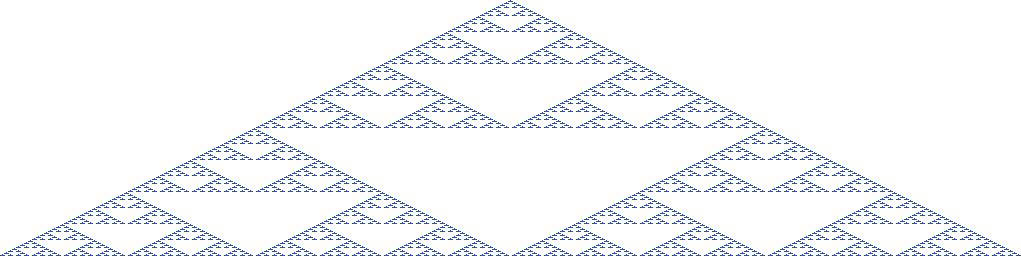
\includegraphics[width=\textwidth]{radius2-fractal}\\[0.5em]
    {\footnotesize\color{muted}The picture drawn by one of the radius-2 rules found by the program
    (\cref{sec:bonus}).}
  \end{center}
  \vfill

  {\large
  \begin{tabular}{@{}>{\color{muted}}l@{\hspace{1.2em}}l@{}}
    Author & \reportauthor \\
    School & Sup Galil\'ee, Universit\'e Sorbonne Paris Nord \\
    Course & Programmation orient\'ee objet (Java), INFO~1, 2023--2024 \\
    Date & \reportdate \\
  \end{tabular}}
  \vspace{0.6cm}
\end{titlepage}


\tableofcontents
\clearpage

\section{Introduction}

A cellular automaton is a grid of cells, each in one of a few states, that evolves in discrete
time: at every step, every cell simultaneously takes a new state computed from the states of its
neighbors by a fixed local rule. The interest of the model lies in the contrast between the
simplicity of the rules and the richness of what they produce: a three-cell rule draws the
Sierpi\'nski triangle, and Conway's Game of Life is capable of universal computation.

The goal of the project is \emph{not} to program one such automaton. It is to design an
architecture able to simulate \emph{any} automaton described in an input file: a grid whose
number of dimensions is only known at run time, neighborhoods that may be predefined or declared
by the user, and an evolution rule written in a small language of nested operators.

This report presents \textbf{Cellula}, the application written to that end. It is a Java~21
program of about 5\,000 lines of code (7\,900 with documentation), with no dependency other than
the JDK, and covered by 409 automated tests. The report follows the order of the subject:

\begin{itemize}
  \item \cref{sec:analysis} reads the subject closely and records the decisions taken where it
    leaves room for interpretation;
  \item \cref{sec:architecture} gives the overall architecture and the class diagram;
  \item \cref{sec:grid,sec:neighborhoods,sec:rules} detail the three entities the subject
    names: the grid, the neighborhoods and the rules;
  \item \cref{sec:definitions} describes the input file format and its validation;
  \item \cref{sec:simulation} covers the simulation, the graphical interface and the menu;
  \item \cref{sec:bonus} answers the bonus question;
  \item \cref{sec:quality} explains how the code is tested and measured.
\end{itemize}

\Cref{fig:teaser} shows the application at work on the two automata the subject requires.

\begin{figure}[H]
  \centering
  \begin{subfigure}[b]{0.52\textwidth}
    \centering
    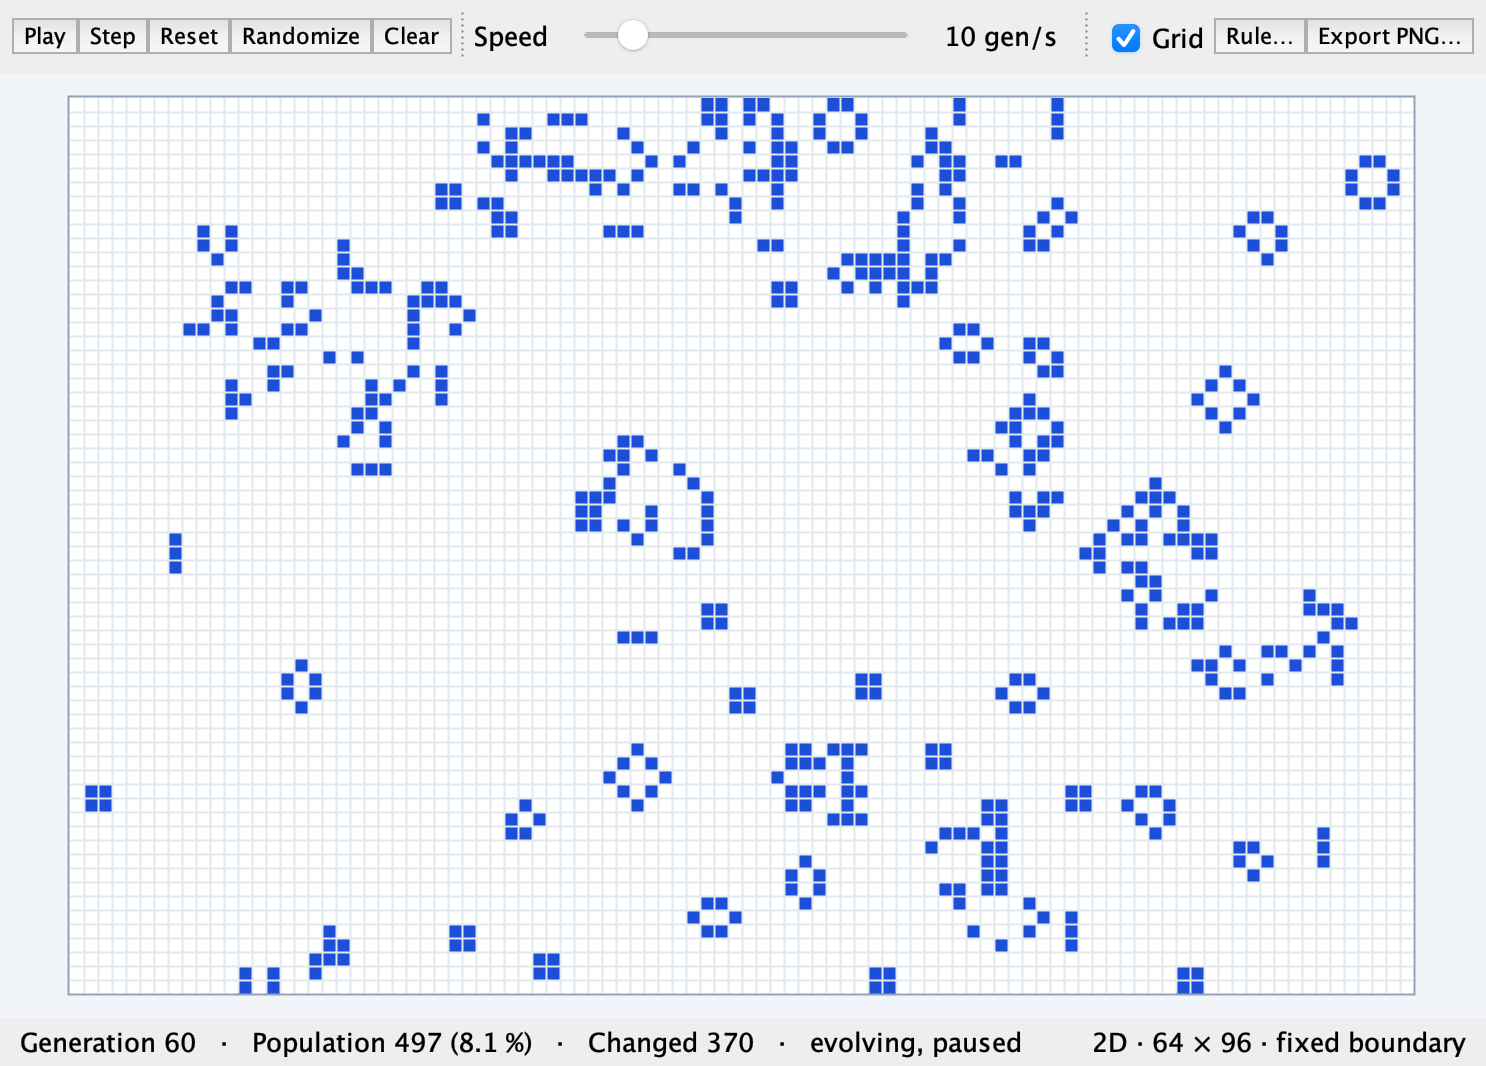
\includegraphics[width=\textwidth]{window-game-of-life}
    \caption{Game of Life, from \code{RANDOM(15)}}
  \end{subfigure}\hfill
  \begin{subfigure}[b]{0.46\textwidth}
    \centering
    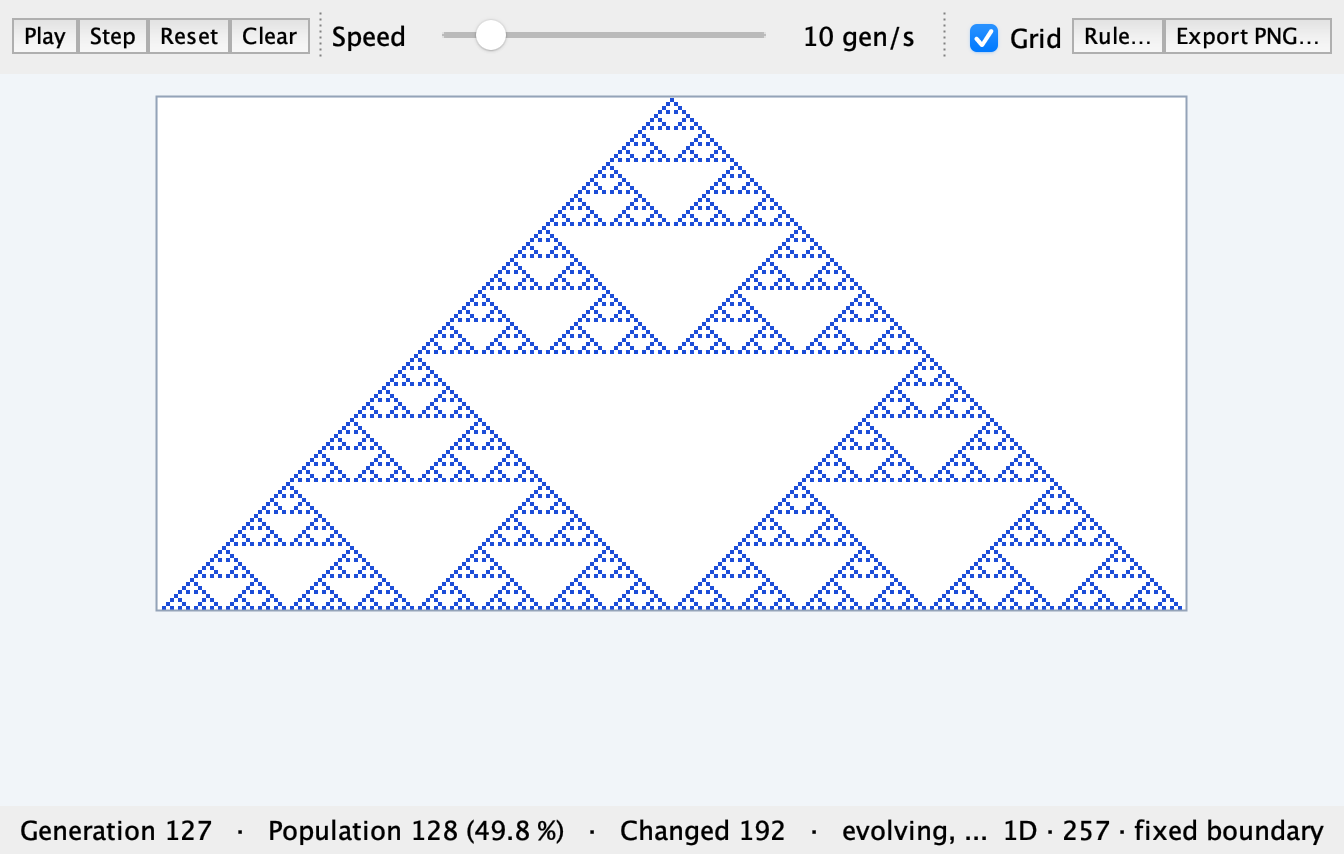
\includegraphics[width=\textwidth]{window-sierpinski}
    \caption{Sierpi\'nski triangle (rule 18)}
  \end{subfigure}
  \caption{The simulation window on the two definition files required by the subject.}
  \label{fig:teaser}
\end{figure}

\section{Analysis of the subject}
\label{sec:analysis}

\subsection{Requirements}

\Cref{tab:requirements} lists what the subject asks for and where each item is realized. Every
requirement is met; the last column of the table doubles as a map of the source code.

\begin{table}[H]
  \centering\small
  \begin{tabularx}{\textwidth}{@{}l L l@{}}
    \toprule
    \S & Requirement & Realized by \\
    \midrule
    2.1 & Recursive array whose dimension is chosen at run time & \code{DynamicArrayND} \\
    2.1 & A class for cells; cells outside the grid are always off & \code{Cell}, \code{VoidCell} \\
    2.2 & Predefined neighborhoods G0, G2, G4, G8, G6, G26 and G$k$* & \code{Neighborhoods} \\
    2.2 & A neighborhood is a rule for traversing cells (\code{Iterable}) & \code{Neighborhood} \\
    2.2 & User-defined neighborhoods given as offsets & \code{NeighborhoodCatalog} \\
    2.3 & The eleven operators, freely nested; a class hierarchy & \code{rule.expression} \\
    2.4 & Display of 1D and 2D automata; 2D slice of 3D+ automata & \code{ui.swing}, \code{Slice} \\
    2.5 & Input file: dimension, size, slice, neighborhoods, rule, initial cells or
          \code{RANDOM(k)} & \code{config} \\
    2.6 & Menu of the input files of the current directory & \code{LauncherFrame} \\
    2.6 & Files for the Game of Life and the Sierpi\'nski triangle & \code{examples/} \\
    2.6.1 & Bonus: a fractal or chaotic rule of radius 2 & \code{explore} \\
    \bottomrule
  \end{tabularx}
  \caption{Requirements of the subject and the code that realizes them.}
  \label{tab:requirements}
\end{table}

\subsection{Decisions on points left open}

The subject leaves several questions open. Each was settled explicitly, and the answer is
documented where the user will look for it.

\paragraph{What does \code{COMPTER} count?} The subject says ``the number of cells in state 1''.
The rule language, however, can produce any integer (through \code{ADD}, for instance), so a
grid may hold other states. \code{COMPTER} was implemented to the letter: it counts cells whose
state is exactly 1. This makes automata with more than two states possible, such as Brian's
Brain where state 1 means ``firing''. Since a cell in state 2 is then invisible to
\code{COMPTER(G0)}, one operator was added, \code{ETAT()}, which returns the state of the cell
itself. It is the only extension to the language and it is redundant for two-state automata.

\paragraph{In which dimension is a predefined neighborhood valid?} The subject states that G2
is ``valid in 1D'', G4 and G8 ``in 2D'', G6 and G26 ``in 3D''. Using G8 on a 3D grid is therefore
an error, reported to the user with the list of valid names. The definition was generalized
rather than restricted (\cref{sec:neighborhoods}): for any dimension $d$, G$2d$ and G$(3^d-1)$
exist, which gives the six names of the subject for $d \le 3$ and sensible ones beyond.

\paragraph{Which display for one dimension?} A one-dimensional grid is a single row of pixels.
The figures of the subject juxtapose the successive states, and this is the display adopted:
time runs down the window.

\paragraph{What if the slice is missing?} The subject requires a file to be \emph{able} to give
the displayed plane of a grid of three dimensions or more. When a file does not, the first two
axes are displayed and the others are pinned at their middle; the plane can then be moved from
the window.

\paragraph{The orientation of coordinates.} Coordinates are array indices from 0. In a picture
the first free axis runs down (rows) and the second to the right (columns), the usual convention
for matrices and the one of Matlab, which the subject refers to for slices.

\paragraph{The example of section 2.3.} The worked example uses G8, which includes the cell
itself, although its text speaks of neighbors. The formula is reproduced verbatim in
\code{examples/subject-example.xml}, and the Game of Life uses G8* as its definition demands.

\subsection{Beyond the subject}

A few features were added because the architecture made them nearly free, and because they make
the program pleasant to use and to verify: a periodic boundary condition, the detection of
convergence and of cycles (both phenomena are described in section 1.2 of the subject), drawing
cells with the mouse, per-state colors, and a command-line interface that runs and pictures
automata without a display. The figures of this report were produced by that interface.

\section{Architecture}
\label{sec:architecture}

\subsection{Guiding principles}

Four principles shaped the design. They are stated here because most of the decisions described
in the following sections derive from them.

\begin{description}[leftmargin=1.2em,style=nextline]
    \item[A pure model.] The classes that \emph{are} the automaton (grid, neighborhoods, rules,
          automaton) know nothing about files, threads or pixels. They form a small library that can be
          tested in isolation and reused behind any front end.
    \item[Dependencies point one way.] Packages form layers (\cref{fig:layers}); a package only
          depends on the layers below it. Swing is confined to a single package: deleting it leaves a
          working batch application.
    \item[Immutability by default.] Positions, shapes, neighborhoods, syntax trees, definitions and
          snapshots are immutable. Mutable state is concentrated in three classes: \code{GridCell},
          \code{CellularAutomaton} and \code{Simulation}.
    \item[Errors are for the user.] Whatever comes from outside is validated at the boundary, and a
          rejected input comes with a message that says what to fix. Inner code then trusts its inputs.
\end{description}

\begin{figure}[H]
    \centering
    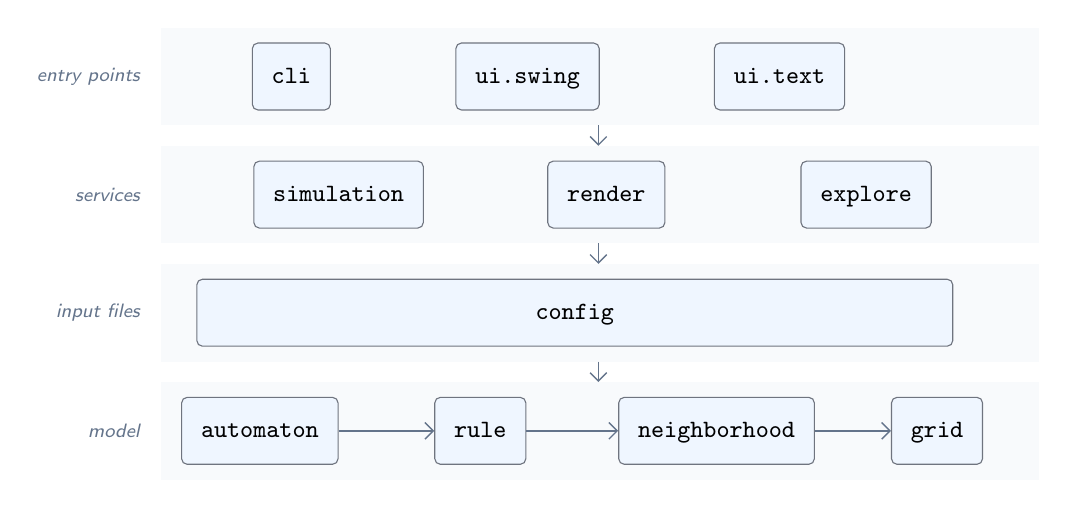
\begin{tikzpicture}[
            box/.style={draw=ink!60, fill=classfill, rounded corners=2pt, minimum height=0.85cm, text height=1.6ex, text depth=0.5ex,
                    font=\ttfamily\small, inner xsep=7pt},
            layer/.style={font=\sffamily\scriptsize\itshape, text=muted, anchor=east},
            dep/.style={-{Straight Barb[length=3pt]}, draw=muted, line width=0.5pt}]
        \node[box] (cli) at (2.0, 4.5) {cli};
        \node[box] (swing) at (5.0, 4.5) {ui.swing};
        \node[box] (text) at (8.2, 4.5) {ui.text};
        \node[box] (sim) at (2.6, 3.0) {simulation};
        \node[box] (render) at (6.0, 3.0) {render};
        \node[box] (explore) at (9.3, 3.0) {explore};
        \node[box, minimum width=9.6cm] (config) at (5.6, 1.5) {config};
        \node[box] (automaton) at (1.6, 0) {automaton};
        \node[box] (rule) at (4.4, 0) {rule};
        \node[box] (nb) at (7.4, 0) {neighborhood};
        \node[box] (grid) at (10.2, 0) {grid};
        \draw[dep] (automaton) -- (rule);
        \draw[dep] (rule) -- (nb);
        \draw[dep] (nb) -- (grid);
        \node[layer] at (0.2, 4.5) {entry points};
        \node[layer] at (0.2, 3.0) {services};
        \node[layer] at (0.2, 1.5) {input files};
        \node[layer] at (0.2, 0) {model};
        \begin{scope}[on background layer]
            \foreach \y in {4.5, 3.0, 1.5, 0}
            \fill[packfill] (0.35, \y - 0.62) rectangle (11.5, \y + 0.62);
            \foreach \y in {3.75, 2.25, 0.75}
            \draw[dep] (5.9, \y + 0.13) -- (5.9, \y - 0.13);
        \end{scope}
    \end{tikzpicture}
    \caption{The packages, in layers. A package depends only on packages of the layers below it
        and, within the model, on the packages to its right.}
    \label{fig:layers}
\end{figure}

\subsection{Overview of the classes}

\Cref{fig:overview} is the class diagram of the project, reduced to the classes that carry the
design and to the relationships between them. Members are omitted here; the diagrams of
\cref{sec:grid,sec:neighborhoods,sec:rules,sec:simulation} give them package by package.

\begin{figure}[H]
    \centering
    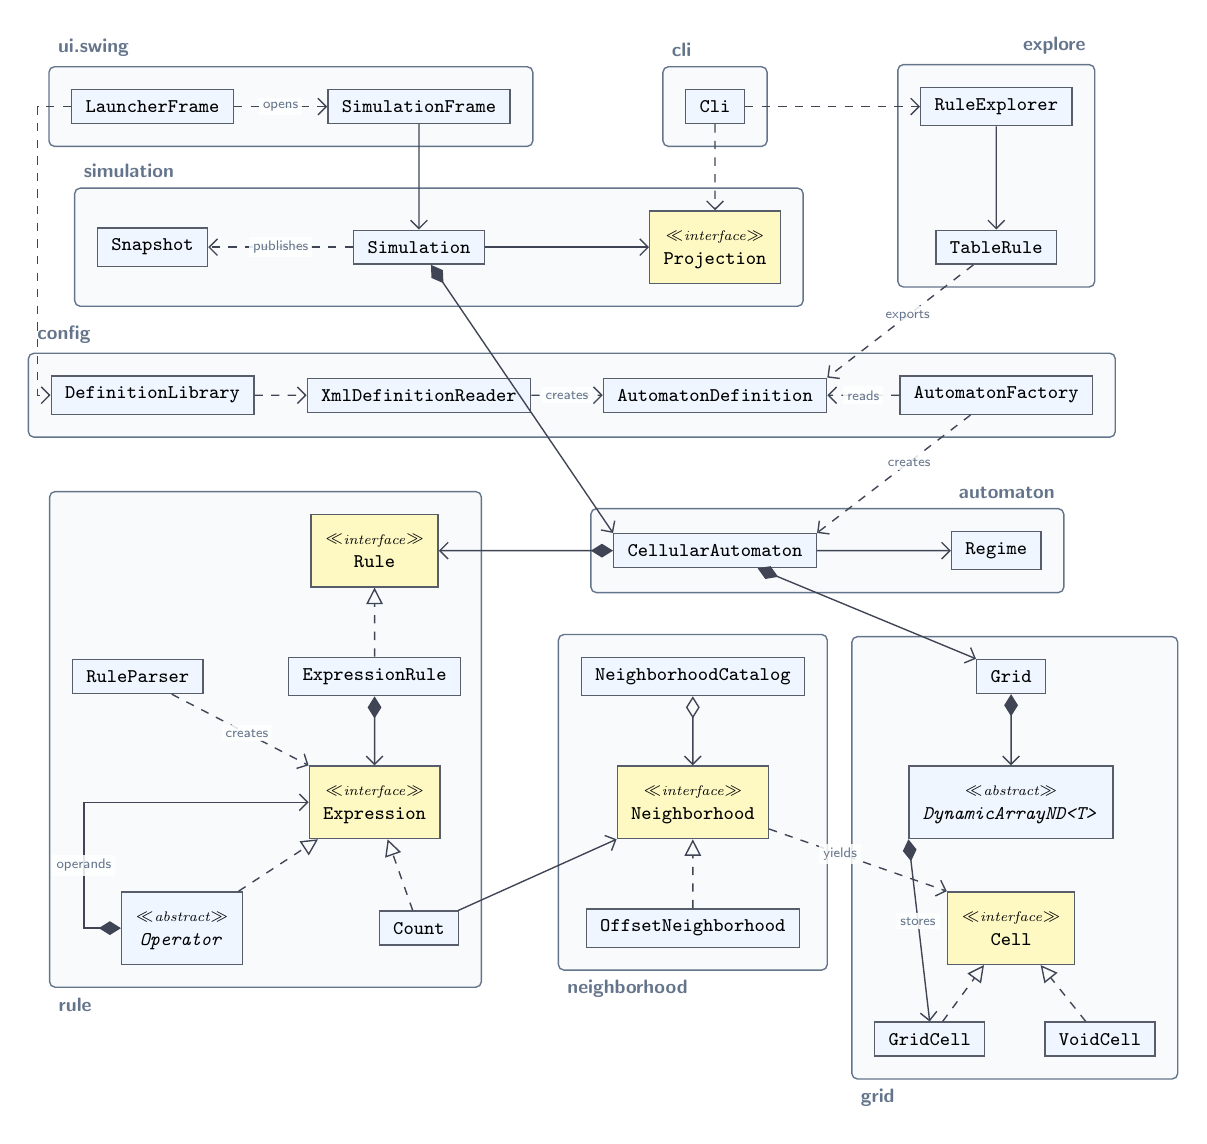
\begin{tikzpicture}[scale=0.94]
        % ---- entry points ---------------------------------------------------------------------
        \node[simple] (launcher) at (0, 0) {LauncherFrame};
        \node[simple] (simframe) at (3.6, 0) {SimulationFrame};
        \node[simple] (cli) at (7.6, 0) {Cli};
        \node[simple] (explorer) at (11.4, 0) {RuleExplorer};
        % ---- simulation -----------------------------------------------------------------------
        \node[simple] (snapshot) at (0, -1.9) {Snapshot};
        \node[simple] (simulation) at (3.6, -1.9) {Simulation};
        \node[simpleiface] (projection) at (7.6, -1.9) {\ctitle[interface]{Projection}};
        \node[simple] (tablerule) at (11.4, -1.9) {TableRule};
        % ---- config ---------------------------------------------------------------------------
        \node[simple] (library) at (0, -3.9) {DefinitionLibrary};
        \node[simple] (reader) at (3.6, -3.9) {XmlDefinitionReader};
        \node[simple] (definition) at (7.6, -3.9) {AutomatonDefinition};
        \node[simple] (factory) at (11.4, -3.9) {AutomatonFactory};
        % ---- automaton ------------------------------------------------------------------------
        \node[simple] (automaton) at (7.6, -6.0) {CellularAutomaton};
        \node[simple] (regime) at (11.4, -6.0) {Regime};
        % ---- rule -----------------------------------------------------------------------------
        \node[simpleiface] (rule) at (3.0, -6.0) {\ctitle[interface]{Rule}};
        \node[simple] (exprule) at (3.0, -7.7) {ExpressionRule};
        \node[simple] (parser) at (-0.2, -7.7) {RuleParser};
        \node[simpleiface] (expression) at (3.0, -9.4) {\ctitle[interface]{Expression}};
        \node[simple] (operator) at (0.4, -11.1) {\atitle{Operator}};
        \node[simple] (count) at (3.6, -11.1) {Count};
        % ---- neighborhood ---------------------------------------------------------------------
        \node[simple] (catalog) at (7.3, -7.7) {NeighborhoodCatalog};
        \node[simpleiface] (neighborhood) at (7.3, -9.4) {\ctitle[interface]{Neighborhood}};
        \node[simple] (offsets) at (7.3, -11.1) {OffsetNeighborhood};
        % ---- grid -----------------------------------------------------------------------------
        \node[simple] (grid) at (11.6, -7.7) {Grid};
        \node[simple] (array) at (11.6, -9.4) {\atitle{DynamicArrayND<T>}};
        \node[simpleiface] (cell) at (11.6, -11.1) {\ctitle[interface]{Cell}};
        \node[simple] (gridcell) at (10.5, -12.6) {GridCell};
        \node[simple] (voidcell) at (12.8, -12.6) {VoidCell};

        % ---- relationships --------------------------------------------------------------------
        \draw[uses] (launcher.west) -- ++(-0.45, 0) |- (library.west);
        \draw[uses] (launcher) -- node[elabel] {opens} (simframe);
        \draw[association] (simframe) -- (simulation);
        \draw[uses] (simulation) -- node[elabel] {publishes} (snapshot);
        \draw[association] (simulation) -- (projection);
        \draw[uses] (cli) -- (projection);
        \draw[uses] (cli) -- (explorer);
        \draw[association] (explorer) -- (tablerule);
        \draw[uses] (tablerule) -- node[elabel, pos=0.45] {exports} (definition.north east);
        \draw[uses] (library) -- (reader);
        \draw[uses] (reader) -- node[elabel] {creates} (definition);
        \draw[uses] (factory) -- node[elabel] {reads} (definition);
        \draw[uses] (factory) -- node[elabel, pos=0.4] {creates} (automaton.north east);
        \draw[composition] (simulation) -- (automaton.north west);
        \draw[composition] (automaton) -- (rule);
        \draw[composition] (automaton) -- (grid.north west);
        \draw[association] (automaton) -- (regime);
        \draw[implements] (exprule) -- (rule);
        \draw[composition] (exprule) -- (expression);
        \draw[uses] (parser) -- node[elabel, pos=0.55] {creates} (expression.north west);
        \draw[implements] (operator) -- (expression);
        \draw[implements] (count) -- (expression);
        \draw[composition] (operator.west) -- ++(-0.5, 0) |- node[elabel, pos=0.25] {operands} (expression.west);
        \draw[association] (count) -- (neighborhood.south west);
        \draw[aggregation] (catalog) -- (neighborhood);
        \draw[implements] (offsets) -- (neighborhood);
        \draw[uses] (neighborhood) -- node[elabel, pos=0.4] {yields} (cell.north west);
        \draw[composition] (grid) -- (array);
        \draw[composition] (array.south west) -- node[elabel, pos=0.45] {stores} (gridcell.north);
        \draw[implements] (gridcell) -- (cell);
        \draw[implements] (voidcell) -- (cell);

        % ---- packages -------------------------------------------------------------------------
        \begin{scope}[on background layer]
            \node[package, fit=(launcher)(simframe)] (p-ui) {};
            \node[package, fit=(cli)] (p-cli) {};
            \node[package, fit=(explorer)(tablerule)] (p-explore) {};
            \node[package, fit=(snapshot)(simulation)(projection)] (p-sim) {};
            \node[package, fit=(library)(reader)(definition)(factory)] (p-config) {};
            \node[package, fit=(automaton)(regime)] (p-automaton) {};
            \node[package, fit=(rule)(parser)(operator)(count)(expression)] (p-rule) {};
            \node[package, fit=(catalog)(neighborhood)(offsets)] (p-nb) {};
            \node[package, fit=(grid)(array)(cell)(gridcell)(voidcell)] (p-grid) {};
        \end{scope}
        \node[packagelabel, anchor=south west] at (p-ui.north west) {ui.swing};
        \node[packagelabel, anchor=south west] at (p-cli.north west) {cli};
        \node[packagelabel, anchor=south east] at (p-explore.north east) {explore};
        \node[packagelabel, anchor=south west] at (p-sim.north west) {simulation};
        \node[packagelabel, anchor=south west] at (p-config.north west) {config};
        \node[packagelabel, anchor=south east] at (p-automaton.north east) {automaton};
        \node[packagelabel, anchor=north west] at (p-rule.south west) {rule};
        \node[packagelabel, anchor=north west] at (p-nb.south west) {neighborhood};
        \node[packagelabel, anchor=north west] at (p-grid.south west) {grid};
    \end{tikzpicture}
    \caption{Class diagram of the project (main classes only).
        \legendarrow{extends}~inheritance,
        \legendarrow{implements}~realization,
        \legendarrow{composition}~composition,
        \legendarrow{aggregation}~aggregation,
        \legendarrow{association}~association,
        \legendarrow{uses}~dependency.}
    \label{fig:overview}
\end{figure}

Reading the diagram from the bottom:

\begin{itemize}
    \item a \code{Grid} stores its cells in a \code{DynamicArrayND}; a \code{Neighborhood} yields
          \code{Cell}s, which are either real \code{GridCell}s or the \code{VoidCell} standing for
          everything outside the grid;
    \item a rule is a tree of \code{Expression}s whose \code{Count} leaves walk neighborhoods; the
          engine only sees it through the one-method interface \code{Rule};
    \item a \code{CellularAutomaton} is composed of a grid and a rule, and reports its
          \code{Regime} (evolving, converged, cycling);
    \item an \code{AutomatonDefinition} is the content of an input file as immutable data; the
          \code{AutomatonFactory} turns it into a live automaton;
    \item a \code{Simulation} runs an automaton on its own thread and publishes \code{Snapshot}s
          to the window.
\end{itemize}

\subsection{Design patterns}

The course presents design patterns as a vocabulary for recurring solutions; \cref{tab:patterns}
lists those that the project uses, each for a reason given in the corresponding section.

\begin{table}[H]
    \centering\small
    \begin{tabularx}{\textwidth}{@{}l l L@{}}
        \toprule
        Pattern                & Where                                                                 & Purpose                                      \\
        \midrule
        Composite              & \code{DynamicArrayND}; \code{Expression}                              & Recursive structures handled
        uniformly                                                                                                                                     \\
        Interpreter            & \code{Expression.evaluate}                                            & The syntax tree of a rule evaluates itself   \\
        Template method        & \code{UnaryOperator}, \code{BinaryOperator}                           & Operand evaluation written
        once                                                                                                                                          \\
        Iterator               & \code{Neighborhood.around}                                            & A neighborhood \emph{is} a traversal         \\
        Strategy               & \code{BoundaryCondition}, \code{Projection}, \code{Rule}              & Interchangeable
        behaviors                                                                                                                                     \\
        Null object, Singleton & \code{VoidCell}                                                       & No bounds checks in rules                    \\
        Factory                & \code{AutomatonFactory}, \code{Neighborhoods}, \code{OperatorCatalog} &
        Construction separated from use                                                                                                               \\
        Builder                & \code{AutomatonDefinition.Builder}                                    & Readable construction of a nine-field record \\
        Observer               & \code{SimulationListener}                                             & The view follows the model without coupling  \\
        Command                & \code{cli.Command}; \code{Simulation}                                 & Uniform dispatch; serialized execution       \\
        \bottomrule
    \end{tabularx}
    \caption{Design patterns used in the project.}
    \label{tab:patterns}
\end{table}

\section{The grid}
\label{sec:grid}

\subsection{A recursive array of any dimension}

In Java the dimension of an array is part of its type: \code{int[][]} has two dimensions and
always will. The subject therefore asks for a data structure whose dimension $d$ is an input of
the program, defined recursively: an array of size $k_1 \times k_2 \times \dots \times k_n$
allocates $k_1$ arrays of size $k_2 \times \dots \times k_n$.

\code{DynamicArrayND<T>} is that structure. The definition has two cases, a recursive one and a
base one, and the class models them with two private subclasses instead of a flag and a pair of
half-used fields:

\begin{itemize}
    \item a \code{Branch} holds a list of arrays that have one dimension less;
    \item a \code{Leaf} is a one-dimensional array and holds the elements.
\end{itemize}

This is the Composite pattern. Client code only sees the abstract type and obtains an instance
from a static factory method, whose signature uses a variable number of arguments, as the subject
suggests:

\begin{lstlisting}
DynamicArrayND<GridCell> cells = DynamicArrayND.create(GridCell::new, 65, 65, 65);
GridCell center = cells.get(32, 32, 32);
\end{lstlisting}

The first argument computes the element stored at given coordinates; it is called once per
element, so an array is never observed half-filled. The construction follows the recursive
definition literally:

\begin{lstlisting}
private static <T> DynamicArrayND<T> allocate(
        Shape shape, int depth, int[] prefix,
        Function<? super Coordinates, ? extends T> initializer) {
    int length = shape.size(depth);
    if (depth == shape.dimension() - 1) {                      // base case: a row of elements
        Object[] elements = new Object[length];
        for (int index = 0; index < length; index++) {
            prefix[depth] = index;
            elements[index] = initializer.apply(Coordinates.of(prefix));
        }
        return new Leaf<>(elements);
    }
    List<DynamicArrayND<T>> children = new ArrayList<>(length);  // recursive case
    for (int index = 0; index < length; index++) {
        prefix[depth] = index;
        children.add(allocate(shape, depth + 1, prefix, initializer));
    }
    return new Branch<>(children);
}
\end{lstlisting}

Access is recursive in the same way. The public method \code{get(int... indices)} checks that
there is one index per dimension, then calls \code{get(indices, 0)}; a \code{Branch} picks the
child designated by \code{indices[depth]} and delegates to it with \code{depth + 1}; a
\code{Leaf} returns the element. An access costs $d$ steps and allocates nothing. The class is
generic and implements \code{Iterable<T>}, visiting elements in row-major order.

\begin{figure}[tbp]
    \centering
    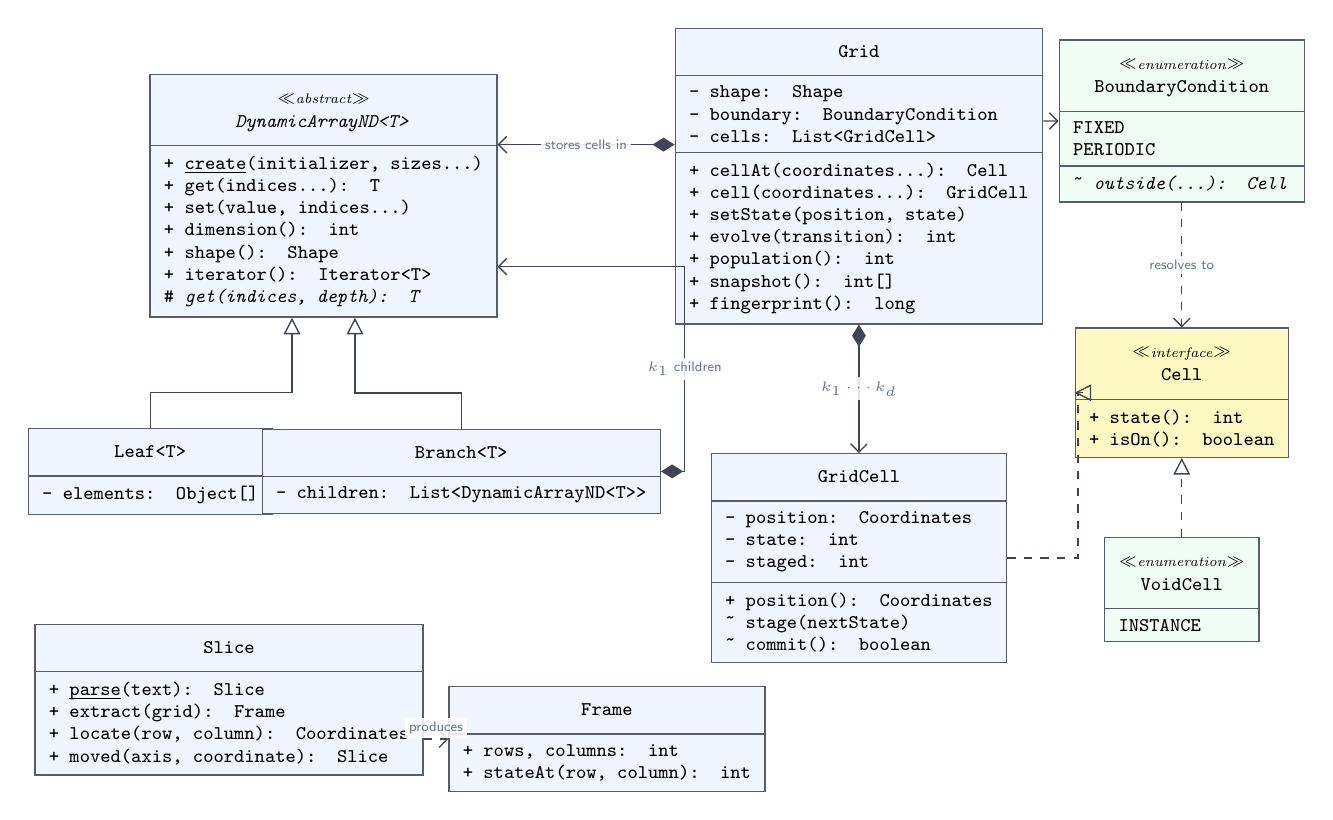
\begin{tikzpicture}
        \node[class] (array) at (0, 0) {\atitle{DynamicArrayND<T>}
            \nodepart{second}+ \static{create}(initializer, sizes...)\\
            + get(indices...): T\\+ set(value, indices...)\\+ dimension(): int\\+ shape(): Shape\\
            + iterator(): Iterator<T>\\\# \textit{get(indices, depth): T}};
        \node[class] (leaf) at (-2.2, -3.5) {\ctitle{Leaf<T>}\nodepart{second}- elements: Object[]};
        \node[class] (branch) at (1.75, -3.5) {\ctitle{Branch<T>}
            \nodepart{second}- children: List<DynamicArrayND<T>>};

        \node[class=3] (grid) at (6.8, 0.25) {\ctitle{Grid}
            \nodepart{second}- shape: Shape\\- boundary: BoundaryCondition\\- cells: List<GridCell>
            \nodepart{third}+ cellAt(coordinates...): Cell\\+ cell(coordinates...): GridCell\\
            + setState(position, state)\\+ evolve(transition): int\\+ population(): int\\
            + snapshot(): int[]\\+ fingerprint(): long};
        \node[enum=3] (boundary) at (10.9, 0.95) {\ctitle[enumeration]{BoundaryCondition}
            \nodepart{second}FIXED\\PERIODIC
            \nodepart{third}\textasciitilde{} \textit{outside(...): Cell}};

        \node[iface] (cell) at (10.9, -2.5) {\ctitle[interface]{Cell}
            \nodepart{second}+ state(): int\\+ isOn(): boolean};
        \node[class=3] (gridcell) at (6.8, -4.6) {\ctitle{GridCell}
            \nodepart{second}- position: Coordinates\\- state: int\\- staged: int
            \nodepart{third}+ position(): Coordinates\\\textasciitilde{} stage(nextState)\\
            \textasciitilde{} commit(): boolean};
        \node[enum] (void) at (10.9, -5.0) {\ctitle[enumeration]{VoidCell}\nodepart{second}INSTANCE};

        \node[class] (slice) at (-1.2, -6.4) {\ctitle{Slice}
            \nodepart{second}+ \static{parse}(text): Slice\\+ extract(grid): Frame\\
            + locate(row, column): Coordinates\\+ moved(axis, coordinate): Slice};
        \node[class] (frame) at (3.6, -6.9) {\ctitle{Frame}
            \nodepart{second}+ rows, columns: int\\+ stateAt(row, column): int};

        \draw[extends] (leaf.north) -- ++(0, 0.45) -| ($(array.south)+(-0.4,0)$);
        \draw[extends] (branch.north) -- ++(0, 0.45) -| ($(array.south)+(0.4,0)$);
        \draw[composition] (branch.east) -- ++(0.3, 0) |- node[elabel, pos=0.25] {$k_1$ children}
        ($(array.east)+(0,-0.9)$);
        \draw[composition] ($(grid.west)+(0,0.4)$) -- node[elabel] {stores cells in}
        ($(array.east)+(0,0.65)$);
        \draw[association] ($(grid.east)+(0,0.7)$) -- (boundary.west);
        \draw[composition] (grid.south) -- node[elabel] {$k_1 \cdots k_d$} (gridcell.north);
        \draw[implements] (gridcell.east) -- ++(0.9, 0) |- (cell.west);
        \draw[implements] (void) -- (cell);
        \draw[uses] (boundary.south) -- node[elabel] {resolves to} (cell.north);
        \draw[uses] (slice.east |- frame.west) -- node[elabel, above] {produces} (frame.west);
    \end{tikzpicture}
    \caption{The \code{grid} package. \code{Shape} and \code{Coordinates}, two small immutable value
        types used throughout, are not drawn.}
    \label{fig:grid}
\end{figure}

\paragraph{Why not a flat array?} A single \code{int[]} indexed by
$i_1 k_2 \cdots k_d + \dots + i_d$ would be more compact and faster. The recursive structure was
kept because the subject asks for it, and it was isolated behind a class of its own: nothing else
in the program knows how cells are stored, so the representation could be swapped without
touching the rest. The measurements of \cref{sec:quality} show that it is fast enough.

\subsection{Cells, and what lies beyond the edge}

A \code{Grid} owns a \code{DynamicArrayND<GridCell>}. Each \code{GridCell} knows its position and
its state (an \code{int}, so that automata are not limited to two states).

Automata are defined on an infinite grid; the subject settles the finite case by stating that any
cell outside the grid is permanently off. Sprinkling bounds checks over every operator would have
been error-prone. Instead, the question ``which cell is at these coordinates?'' always has an
answer:

\begin{lstlisting}
public Cell cellAt(int... coordinates) {
    if (shape.contains(coordinates)) {
        return storage.get(coordinates);
    }
    return boundary.outside(this, coordinates);
}
\end{lstlisting}

Rules see cells through the two-method interface \code{Cell}. Outside the grid, the
\code{FIXED} boundary answers with \code{VoidCell.INSTANCE}, a cell whose state is 0 forever: a
Null Object, implemented as a single-element enumeration, which is the idiomatic Java singleton.
The boundary condition itself is a Strategy written as an enumeration with one method body per
constant; the second constant, \code{PERIODIC}, wraps coordinates around and turns the grid into
a torus. No rule, operator or neighborhood contains a bounds check.

\subsection{Simultaneous evolution}

``All the cells of a cellular automaton evolve simultaneously.'' Updating cells in place, one
after the other, would let a cell read the \emph{new} state of a neighbor updated before it and
silently compute a different automaton. The grid owns the protocol that prevents this:

\begin{lstlisting}
public int evolve(ToIntFunction<? super GridCell> transition) {
    if (cells.size() >= PARALLEL_THRESHOLD) {
        cells.parallelStream().forEach(cell -> cell.stage(transition.applyAsInt(cell)));
    } else {
        for (GridCell cell : cells) {
            cell.stage(transition.applyAsInt(cell));
        }
    }
    int changed = 0;
    for (GridCell cell : cells) {
        if (cell.commit()) {
            changed++;
        }
    }
    return changed;
}
\end{lstlisting}

In the first phase every cell computes its next state from the untouched current generation and
\emph{stages} it in a private field; in the second, all cells \emph{commit}. \code{stage} and
\code{commit} are package-private: only the grid can call them, so the invariant cannot be broken
from outside.

The first phase only reads shared state and writes one private field per cell. It is therefore
safe to run on several threads, which the grid does for 8\,192 cells or more, using a parallel
stream over the flat list of cells built once at construction. The number of changed cells,
returned for free by the second phase, is what detects convergence.

A unit test pins the property down: with the transition ``copy your left neighbor'', a row
\code{1 0 0 0 0} must become \code{0 1 0 0 0}, not \code{1 1 1 1 1}.

\subsection{Slices}

A grid of three dimensions or more is displayed through a plane. \code{Slice} parses the
Matlab-like notation of the subject, \code{(37, :, :)}, where a colon marks a displayed axis, and
\code{extract(grid)} returns the selected plane as a \code{Frame}, an immutable two-dimensional
picture of states. The same class handles the degenerate cases, \code{(:, :)} for a 2D grid and
\code{(:)} for a 1D one, so the display code is identical in every dimension.

\section{Neighborhoods}
\label{sec:neighborhoods}

\subsection{A neighborhood is a traversal}

The subject is explicit: ``a neighborhood is nothing but a rule for traversing the cells
neighboring a given cell'', and it points to \code{Iterator} and \code{Iterable}. The interface
says exactly that:

\begin{lstlisting}
public interface Neighborhood {
    String name();
    int dimension();
    int size();
    Iterable<Cell> around(Grid grid, GridCell center);
}
\end{lstlisting}

An operator consumes a neighborhood with a \code{for} loop and never manipulates a coordinate.
This is the whole implementation of \code{COMPTER}:

\begin{lstlisting}
public int evaluate(EvaluationContext context) {
    int count = 0;
    for (Cell neighbor : neighborhood.around(context.grid(), context.cell())) {
        if (neighbor.isOn()) {
            count++;
        }
    }
    return count;
}
\end{lstlisting}

\code{OffsetNeighborhood} is the one implementation the project needs. It holds the list of the
coordinates of the neighbors of a cell located at the origin, which is precisely how the subject
writes neighborhoods: $G4^* = \{(-1, 0), (1, 0), (0, -1), (0, 1)\}$. Its iterator adds each
offset to the position of the center and asks the grid for the cell there:

\begin{lstlisting}
public Cell next() {
    if (!hasNext()) {
        throw new NoSuchElementException();
    }
    int[] delta = deltas[next++];
    for (int axis = 0; axis < dimension; axis++) {
        cursor[axis] = center.get(axis) + delta[axis];
    }
    return grid.cellAt(cursor);     // the grid resolves positions beyond its edges
}
\end{lstlisting}

The iterator reuses one buffer for all the neighbors, so walking a neighborhood allocates two
small objects however many cells it visits. Because \code{Grid.cellAt} always returns a cell
(\cref{sec:grid}), a walk yields exactly \code{size()} cells even in a corner of the grid.

\begin{figure}[tbp]
  \centering
  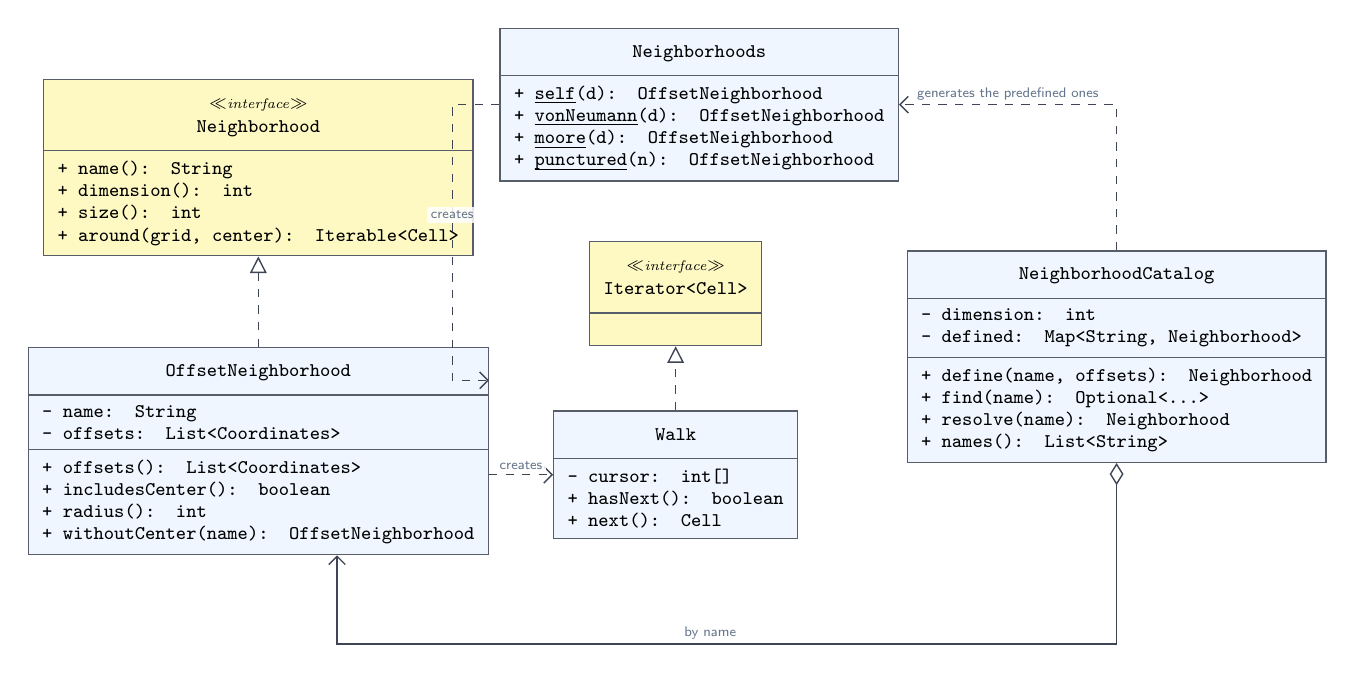
\begin{tikzpicture}
    \node[iface] (nb) at (0, 0) {\ctitle[interface]{Neighborhood}
      \nodepart{second}+ name(): String\\+ dimension(): int\\+ size(): int\\
        + around(grid, center): Iterable<Cell>};
    \node[class=3] (off) at (0, -3.6) {\ctitle{OffsetNeighborhood}
      \nodepart{second}- name: String\\- offsets: List<Coordinates>
      \nodepart{third}+ offsets(): List<Coordinates>\\+ includesCenter(): boolean\\
        + radius(): int\\+ withoutCenter(name): OffsetNeighborhood};
    \node[class] (walk) at (5.3, -3.9) {\ctitle{Walk}
      \nodepart{second}- cursor: int[]\\+ hasNext(): boolean\\+ next(): Cell};
    \node[iface] (iter) at (5.3, -1.6) {\ctitle[interface]{Iterator<Cell>}};
    \node[class] (factory) at (5.6, 0.8) {\ctitle{Neighborhoods}
      \nodepart{second}+ \static{self}(d): OffsetNeighborhood\\
        + \static{vonNeumann}(d): OffsetNeighborhood\\
        + \static{moore}(d): OffsetNeighborhood\\
        + \static{punctured}(n): OffsetNeighborhood};
    \node[class=3] (catalog) at (10.9, -2.4) {\ctitle{NeighborhoodCatalog}
      \nodepart{second}- dimension: int\\- defined: Map<String, Neighborhood>
      \nodepart{third}+ define(name, offsets): Neighborhood\\+ find(name): Optional<...>\\
        + resolve(name): Neighborhood\\+ names(): List<String>};

    \draw[implements] (off) -- (nb);
    \draw[implements] (walk) -- (iter);
    \draw[uses] (off.east |- walk.west) -- node[elabel, above] {creates} (walk.west);
    \draw[uses] (catalog.north) |- node[elabel, pos=0.75, above] {generates the predefined ones}
      (factory.east);
    \draw[uses] (factory.west) -- ++(-0.6, 0) |- node[elabel, pos=0.2] {creates}
      ($(off.east)+(0,0.9)$);
    \draw[aggregation] (catalog.south) |- ++(-2, -2.3) -| node[elabel, pos=0.2, above] {by name}
      ($(off.south)+(1.0,0)$);
  \end{tikzpicture}
  \caption{The \code{neighborhood} package. \code{Walk} is the private iterator of
    \code{OffsetNeighborhood}.}
  \label{fig:neighborhood}
\end{figure}

\subsection{Six names, two formulas}

The subject lists six predefined neighborhoods. Writing six classes, or six hard-coded lists of
offsets, would duplicate what is really two definitions that make sense in every dimension $d$:

\begin{center}\small
  \begin{tabular}{@{}llccccc@{}}
    \toprule
    Family & Neighbors of a cell & Count & $d = 1$ & $d = 2$ & $d = 3$ & $d = 4$ \\
    \midrule
    von Neumann & those sharing a face & $2d$ & G2 & G4 & G6 & G8 \\
    Moore & those sharing a face, an edge or a corner & $3^d - 1$ & G2 & G8 & G26 & G80 \\
    \bottomrule
  \end{tabular}
\end{center}

The names of the subject turn out to be the number of neighbors. \code{Neighborhoods} generates
both families for any $d$: the von Neumann offsets are the $2d$ unit vectors, and the Moore
offsets are enumerated by an odometer over $\{-1, 0, 1\}^d$. \code{G0} is the cell alone, and
the starred variant of a neighborhood is obtained by removing the origin from its offsets.

\subsection{Resolving names}

A rule refers to neighborhoods by name. \code{NeighborhoodCatalog}, created for the dimension of
the grid, resolves those names:

\begin{itemize}
  \item a name declared in the input file designates the user's neighborhood;
  \item otherwise \code{G0} is the cell alone, \code{G}$\langle 2d \rangle$ the von Neumann
    neighborhood and \code{G}$\langle 3^d - 1 \rangle$ the Moore neighborhood, each with a
    starred variant;
  \item any other name is an error.
\end{itemize}

This reproduces the validity rules of the subject (G4 and G8 only in 2D, G6 and G26 only in 3D)
without a table of special cases, and it extends them: on a four-dimensional grid, \code{G8}
designates the eight face neighbors and \code{G80} the full neighborhood. The same name may thus
mean different things in different dimensions, which is why a catalog is bound to one dimension.

User-defined neighborhoods are checked when they are declared: the name must follow the
convention of the subject (a capital G, a number, an optional star), and every offset must have
as many coordinates as the grid has dimensions. An unknown name is reported with the names that
do exist:

\begin{lstlisting}[style=text]
unknown neighborhood 'G26' for a 2-dimensional grid (available: G0, G4, G4*, G8, G8*)
\end{lstlisting}

\section{Rules}
\label{sec:rules}

\subsection{From a formula to a tree}

The subject defines rules as compositions of eleven operators, where an argument is either a
number or the result of another operator, and one operator, \code{COMPTER}, takes a neighborhood.
The worked example of the subject is

\begin{lstlisting}[style=rule]
SI(EQ(COMPTER(G0), 1),
   SI(SUPEQ(COMPTER(G8), 4), 0, 1),
   SI(EQ(COMPTER(G8), 2), 1, 0))
\end{lstlisting}

Such a formula is a tree: operators are inner nodes, numbers and counts are leaves
(\cref{fig:tree}). The program parses the text of a rule \emph{once} into that tree, then
evaluates the tree for every cell at every step.

\begin{figure}[H]
  \centering
  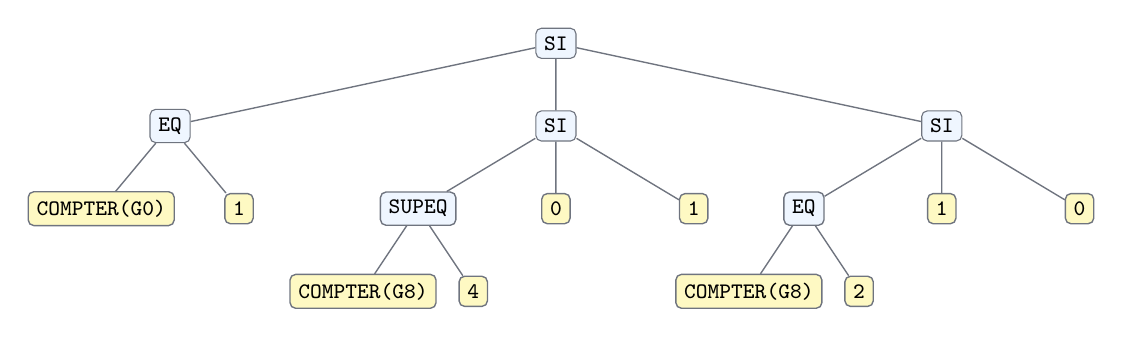
\begin{tikzpicture}[
      level distance=1.05cm, sibling distance=1.9cm,
      every node/.style={font=\ttfamily\footnotesize, draw=ink!60, fill=classfill,
        rounded corners=2pt, inner sep=3pt},
      leaf/.style={fill=ifacefill},
      edge from parent/.style={draw=ink!60, line width=0.5pt},
      level 1/.style={sibling distance=4.9cm},
      level 2/.style={sibling distance=1.75cm},
      level 3/.style={sibling distance=1.4cm}]
    \node {SI}
      child {node {EQ}
        child {node[leaf] {COMPTER(G0)}}
        child {node[leaf] {1}}}
      child {node {SI}
        child {node {SUPEQ}
          child {node[leaf] {COMPTER(G8)}}
          child {node[leaf] {4}}}
        child {node[leaf] {0}}
        child {node[leaf] {1}}}
      child {node {SI}
        child {node {EQ}
          child {node[leaf] {COMPTER(G8)}}
          child {node[leaf] {2}}}
        child {node[leaf] {1}}
        child {node[leaf] {0}}};
  \end{tikzpicture}
  \caption{The syntax tree of the example of the subject.}
  \label{fig:tree}
\end{figure}

\subsection{The hierarchy of operators}

The subject advises to ``think carefully about the class hierarchy used to represent the
operators''. \Cref{fig:rule} shows the one that was chosen.

\begin{figure}[tbp]
  \centering
  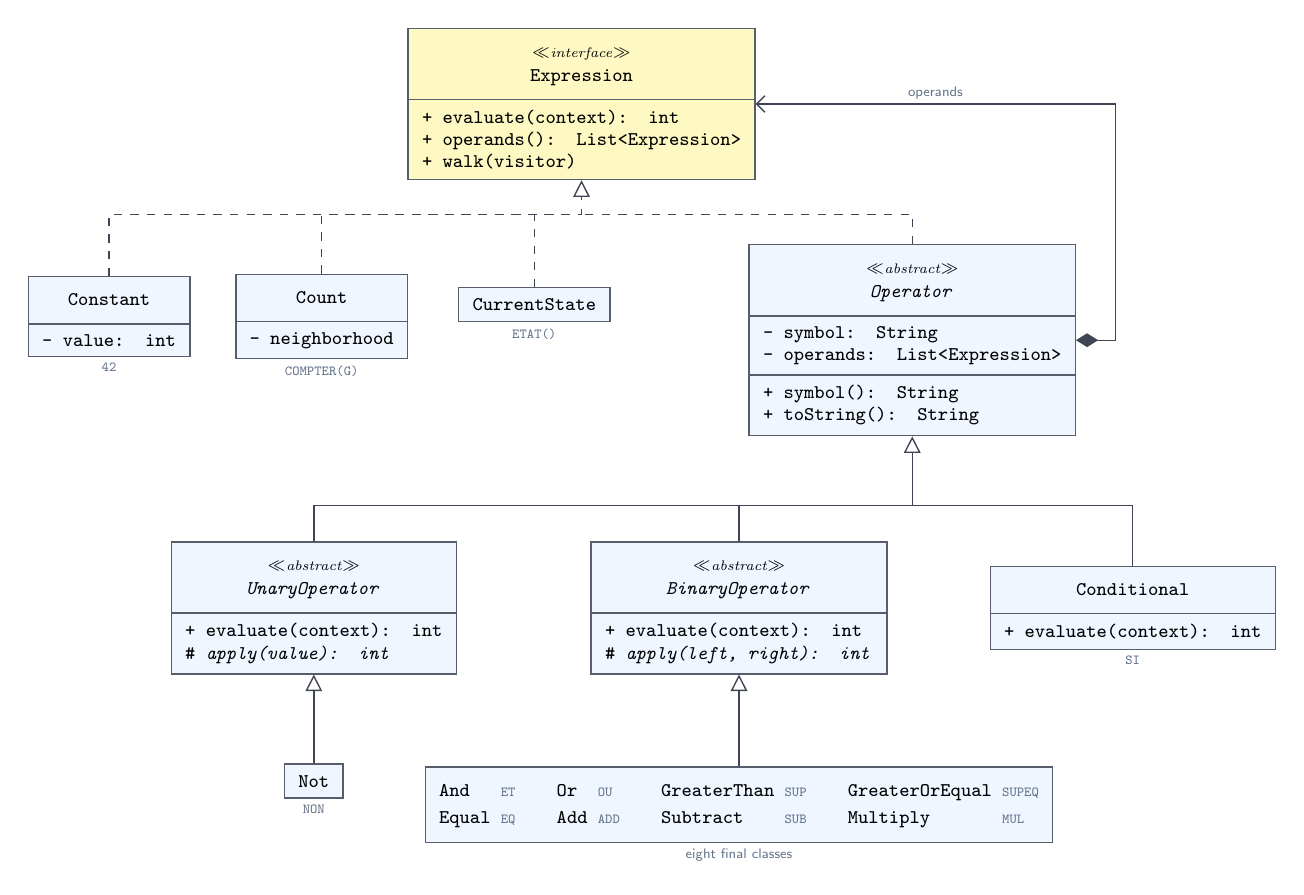
\begin{tikzpicture}[kw/.style={font=\ttfamily\tiny, text=muted, inner sep=2pt}]
    \node[iface] (expr) at (0, 0) {\ctitle[interface]{Expression}
      \nodepart{second}+ evaluate(context): int\\+ operands(): List<Expression>\\
        + walk(visitor)};
    \node[class, label={[kw]below:42}] (const) at (-6.0, -2.7)
      {\ctitle{Constant}\nodepart{second}- value: int};
    \node[class, label={[kw]below:COMPTER(G)}] (count) at (-3.3, -2.7)
      {\ctitle{Count}\nodepart{second}- neighborhood};
    \node[simple, label={[kw]below:ETAT()}] (state) at (-0.6, -2.55) {\textbf{CurrentState}};
    \node[class=3] (op) at (4.2, -3.0) {\atitle{Operator}
      \nodepart{second}- symbol: String\\- operands: List<Expression>
      \nodepart{third}+ symbol(): String\\+ toString(): String};
    \node[class] (unary) at (-3.4, -6.4) {\atitle{UnaryOperator}
      \nodepart{second}+ evaluate(context): int\\\# \textit{apply(value): int}};
    \node[class] (binary) at (2.0, -6.4) {\atitle{BinaryOperator}
      \nodepart{second}+ evaluate(context): int\\\# \textit{apply(left, right): int}};
    \node[class, label={[kw]below:SI}] (cond) at (7.0, -6.4) {\ctitle{Conditional}
      \nodepart{second}+ evaluate(context): int};
    \node[simple, label={[kw]below:NON}] (not) at (-3.4, -8.6) {\textbf{Not}};
    \node[simple] (binaries) at (2.0, -8.9) {%
      \begin{tabular}{@{}l@{\ }l@{\qquad}l@{\ }l@{\qquad}l@{\ }l@{\qquad}l@{\ }l@{}}
        \textbf{And} & {\tiny\color{muted}ET} & \textbf{Or} & {\tiny\color{muted}OU} &
        \textbf{GreaterThan} & {\tiny\color{muted}SUP} &
        \textbf{GreaterOrEqual} & {\tiny\color{muted}SUPEQ} \\
        \textbf{Equal} & {\tiny\color{muted}EQ} & \textbf{Add} & {\tiny\color{muted}ADD} &
        \textbf{Subtract} & {\tiny\color{muted}SUB} &
        \textbf{Multiply} & {\tiny\color{muted}MUL}
      \end{tabular}};
    \node[kw, anchor=north] at (binaries.south) {\normalfont\sffamily eight final classes};

    \coordinate (bus) at (0, -1.4);
    \draw[implements] (const.north) |- (bus) -- (expr.south);
    \draw[ink!80, dashed, line width=0.5pt] (count.north) |- (bus);
    \draw[ink!80, dashed, line width=0.5pt] (state.north) |- (bus);
    \draw[ink!80, dashed, line width=0.5pt] (op.north) |- (bus);
    \draw[composition] (op.east) -- ++(0.5, 0) |- node[elabel, pos=0.75, above] {operands}
      (expr.east);

    \coordinate (bus2) at (4.2, -5.1);
    \draw[extends] (binary.north) |- (bus2) -- (op.south);
    \draw[ink!80, line width=0.5pt] (unary.north) |- (bus2);
    \draw[ink!80, line width=0.5pt] (cond.north) |- (bus2);
    \draw[extends] (not) -- (unary);
    \draw[extends] (binaries) -- (binary);
  \end{tikzpicture}
  \caption{The \code{rule.expression} package: the class hierarchy of the operators, with the
    keyword of each in gray.}
  \label{fig:rule}
\end{figure}

\paragraph{One interface.} Every node, leaf or operator, is an \code{Expression} and can
evaluate itself for a cell: this is the Composite pattern used as an Interpreter. The engine
never asks a node what kind it is.

\paragraph{Grouping by arity.} Operators differ in what they compute, not in how they obtain
their arguments. The abstract classes \code{UnaryOperator} and \code{BinaryOperator} evaluate the
operands and delegate the computation to an abstract method, which is the Template Method
pattern:

\begin{lstlisting}
public abstract class BinaryOperator extends Operator {
    @Override
    public final int evaluate(EvaluationContext context) {
        return apply(left.evaluate(context), right.evaluate(context));
    }

    protected abstract int apply(int left, int right);
}
\end{lstlisting}

A concrete operator is then reduced to its definition in the subject. Here is \code{ET},
complete:

\begin{lstlisting}
/** ET(a, b): yields 1 if both operands are different from 0, and 0 otherwise. */
public final class And extends BinaryOperator {
    public static final String SYMBOL = "ET";

    public And(Expression left, Expression right) {
        super(SYMBOL, left, right);
    }

    @Override
    protected int apply(int left, int right) {
        return left != 0 && right != 0 ? 1 : 0;
    }
}
\end{lstlisting}

\paragraph{What the common superclass buys.} \code{Operator} stores the keyword and the operands
and implements, once, everything that depends on structure alone: printing in canonical form,
equality, and traversal. Printing then parsing a tree gives an equal tree, a property the tests
check.

\paragraph{The exceptions.} \code{Conditional} (\code{SI}) does not fit the template on purpose:
it evaluates only the branch it selects, which spares whole sub-trees. \code{Count} is not an
\code{Operator} at all, since its argument is a neighborhood and not a value; the type system
thereby rules out nonsense such as \code{ADD(G8, 1)}.

\paragraph{Purity.} Expressions are immutable and evaluation has no side effect. Evaluation
order is therefore unobservable, a single tree can be evaluated for many cells at the same time
by several threads (\cref{sec:grid}), and the laziness of \code{SI} cannot change a result.

\subsection{The parser}

Rules are parsed by a hand-written lexer and recursive-descent parser; the language is small
enough that a parser generator would have been a dependency for no benefit. The grammar is:

\begin{lstlisting}[style=text]
rule         := expression END
expression   := NUMBER | NAME '(' arguments ')'
arguments    := neighborhood                        -- for COMPTER
              | [ expression { ',' expression } ]   -- for every other operator
neighborhood := NAME                                -- G0, G8*, ...
\end{lstlisting}

The \code{Lexer} turns the text into tokens that remember their position. A name may end with a
star, which is what makes \code{G8*} a single token. The \code{RuleParser} has one method per
production.

The parser knows no operator. When it meets a name, it asks an \code{OperatorCatalog} for the
\emph{signature} of that keyword, which says how to read the arguments and how to build the
node. Signatures form a sealed interface with two implementations, so the compiler checks that
the parser handles both:

\begin{lstlisting}
Expression node = switch (signature) {
    case NeighborhoodOperator operator -> operator.factory().apply(neighborhood(operator));
    case ValueOperator operator -> {
        List<Expression> arguments = arguments();
        if (arguments.size() != operator.arity()) {
            throw error(name, operator.symbol() + " expects " + operator.arity()
                    + " argument(s) but got " + arguments.size());
        }
        yield operator.factory().apply(arguments);
    }
};
\end{lstlisting}

The catalog is the single place where a keyword is bound to a class:

\begin{lstlisting}
catalog.register(binary(And.SYMBOL, And::new), "AND");
catalog.register(new NeighborhoodOperator(Count.SYMBOL, Count::new), "COUNT");
\end{lstlisting}

Adding an operator to the language thus takes one class of about ten lines and one line of
registration; arity checking, error messages and printing follow. Keywords are case-insensitive
and each has an English alias.

Neighborhood names are resolved \emph{during} parsing, against the catalog of the grid's
dimension (\cref{sec:neighborhoods}). A tree that parses is therefore guaranteed to be
evaluable: no error can occur later, in the middle of a simulation.

\subsection{Error messages}

A rule is text typed by a person, and mistakes are the normal case. Every syntax error carries
the position of the faulty token (class \code{RuleSyntaxException}), and its message quotes the
line and points at the culprit:

\begin{lstlisting}[style=text]
unknown neighborhood 'G9' for a 2-dimensional grid (available: G0, G4, G4*, G8, G8*) (line 2, column 12)
       COMPTER(G9),
               ^
\end{lstlisting}

Eighteen distinct mistakes (missing parenthesis, wrong number of arguments, unknown operator, a
neighborhood used as a value, \ldots) are covered by a parameterized test that checks both the
message and the reported position.

\section{Definition files}
\label{sec:definitions}

\subsection{The format}

The subject leaves the format open and suggests XML. XML was adopted: the JDK ships a parser and
a schema validator, so the choice costs no dependency and brings structural validation for free.
\Cref{lst:definition} is a complete definition; it carries the six pieces of information required
by section 2.5 of the subject, in the notations the subject itself uses.

\begin{lstlisting}[style=xml, caption={A definition file using every feature of the format.},
  label={lst:definition}, captionpos=b]
<automaton name="Everything at once">
  <description>A 3D automaton that uses every feature of the format.</description>
  <dimension>3</dimension>                        <!-- dimensionality of the grid -->
  <size>40, 40, 40</size>                         <!-- one extent per dimension -->
  <boundary>periodic</boundary>                   <!-- extension; default: fixed -->
  <slice>(20, :, :)</slice>                       <!-- displayed plane, for 3D and more -->
  <neighborhoods>                                 <!-- additional neighborhoods -->
    <neighborhood name="G3">{(0, 0, 0), (1, 1, 0), (-1, 0, 0)}</neighborhood>
  </neighborhoods>
  <rule>                                          <!-- the evolution rule -->
    SI(EQ(COMPTER(G0), 1),
       SUPEQ(COMPTER(G26*), 13),
       EQ(COMPTER(G3), 2))
  </rule>
  <initial seed="42">RANDOM(50)</initial>         <!-- or a list of coordinates -->
  <colors>                                        <!-- extension -->
    <state value="0" color="#0F172A"/>
    <state value="1" color="#38BDF8"/>
  </colors>
</automaton>
\end{lstlisting}

The elements may come in any order. \code{boundary}, \code{slice}, \code{neighborhoods},
\code{colors} and \code{description} are optional. Coordinates and sets of coordinates are
written as in the subject; on a one-dimensional grid the parentheses may be dropped, so the
initial state of the Sierpi\'nski file is simply \code{(128)}.

\subsection{Three stages of validation}

A file written by hand will contain mistakes, and the worst way to learn about them is an
exception in the middle of a simulation. \code{XmlDefinitionReader} therefore accepts a file only
after three successive checks, each catching a different class of errors.

\begin{enumerate}
    \item \textbf{Structure.} The document is validated against an XML Schema bundled with the
          application (\code{automaton.xsd}): unknown or duplicated elements, missing mandatory ones,
          malformed colors or neighborhood names. These errors come with a line number.
    \item \textbf{Consistency.} The values are parsed and cross-checked: as many sizes as
          dimensions, a slice that fits the grid and leaves exactly two free axes, offsets and initial
          cells that have the right number of coordinates and lie inside the grid.
    \item \textbf{The rule.} The rule is compiled against the neighborhoods of the file. This proves
          that it is syntactically correct and only refers to neighborhoods that exist in the grid's
          dimension.
\end{enumerate}

A file that passes is guaranteed to be instantiable. A file that fails yields a
\code{DefinitionException}, a checked exception because every caller has to do something about
it, whose message starts with the name of the file. Twenty-seven kinds of invalid files are
exercised by a parameterized test.

\paragraph{Security.} A definition file may come from someone else. The XML parser is configured
to refuse document type declarations and external entities, which closes the classic XML external
entity attack; a test feeds it such a document. The size of a grid and the nesting depth of a
rule are bounded, so a hostile file cannot exhaust the memory or the stack.

\subsection{A definition is data}

The reader does not build an automaton. It builds an \code{AutomatonDefinition}, an immutable
record holding the sizes, the offsets of the neighborhoods, the rule \emph{as text} and the
initial state. Turning it into live objects is the separate job of \code{AutomatonFactory}:

\begin{lstlisting}
public static CellularAutomaton create(AutomatonDefinition definition) {
    ExpressionRule rule = compileRule(definition);
    Grid grid = new Grid(definition.shape(), definition.boundary());
    definition.initialState().applyTo(grid);
    return new CellularAutomaton(grid, rule);
}
\end{lstlisting}

This intermediate form is what the rest of the application manipulates. The menu displays
definitions without allocating any grid; a simulation instantiates one; the tests and the rule
explorer build definitions in code with a Builder, since the record has nine components:

\begin{lstlisting}
AutomatonDefinition glider = AutomatonDefinition.builder()
        .name("Glider")
        .size(20, 20)
        .boundary(BoundaryCondition.PERIODIC)
        .rule("SI(COMPTER(G0), OU(EQ(COMPTER(G8*), 2), EQ(COMPTER(G8*), 3)), EQ(COMPTER(G8*), 3))")
        .initialState(new InitialState.ExplicitCells(cells))
        .build();
\end{lstlisting}

The two forms of initial state allowed by the subject are the two implementations of a sealed
interface, \code{InitialState}: \code{ExplicitCells} and \code{RandomFill}. A sealed interface
states in the code that there are exactly two cases and lets the compiler verify that both are
handled. An \code{XmlDefinitionWriter} does the inverse of the reader, and a test checks that
writing then reading a definition gives back an equal definition.

\subsection{The files of a directory}

The menu required by the subject lists ``all the input files of the current directory''.
\code{DefinitionLibrary} scans a directory for XML files whose root element is
\code{<automaton>}, which keeps unrelated XML files (the \code{pom.xml} of the project, for one)
out of the menu. Each file becomes an \code{Entry}, another sealed interface: \code{Loaded} with
its definition, or \code{Broken} with the reason of the rejection. Invalid files are thus listed
with an explanation instead of silently disappearing.

\section{Simulation and user interface}
\label{sec:simulation}

\subsection{The automaton}

\code{CellularAutomaton} is the composition announced by the subject: a grid, a rule and a
discrete clock. One call to \code{step()} is one tick:

\begin{lstlisting}
public StepReport step() {
    int changed = grid.evolve(cell -> rule.nextState(grid, cell));
    generation++;
    if (changed == 0) {
        regime = Regime.FIXED_POINT;
    } else {
        int period = cycles.observe(grid.fingerprint(), generation);
        regime = period >= 2 ? Regime.cycle(period) : Regime.TRANSIENT;
    }
    return new StepReport(generation, changed, regime);
}
\end{lstlisting}

The automaton depends on the one-method interface \code{Rule}, not on the rule language: the
tests drive it with lambdas, and the expression trees of \cref{sec:rules} are plugged in through
the adapter \code{ExpressionRule}.

Section 1.2 of the subject describes two long-term behaviors: the grid may become ``identical
between two time steps'' (the automaton has \emph{converged}), or show ``periodic patterns that
repeat''. The automaton detects both and reports them as its \code{Regime}. Convergence is a step
that changed no cell. For cycles, a \code{CycleDetector} remembers a 64-bit fingerprint of each
of the last 1\,024 generations; since the evolution is deterministic, meeting a known fingerprint
again means that the automaton has entered a cycle whose period is the distance between the two
sightings. Remembering fingerprints rather than grids costs eight bytes per generation whatever
the size of the grid. On the \code{glider.xml} example, a glider travelling on a
$20 \times 20$ torus, the window announces a ``cycle of period 80'' at generation 80.

\subsection{Threading model}

A generation of a large grid takes tens of milliseconds, and a user interface must never wait
that long. The automaton therefore does not run on the Swing thread. \code{Simulation} owns one
background thread and \emph{confines} the automaton to it (\cref{fig:threads}):

\begin{itemize}
  \item every public method (\code{play}, \code{pause}, \code{step}, \code{reset},
    \code{setCell}, \code{setSlice}, \ldots) merely posts a command to that thread and returns;
  \item commands are executed one after the other, in order, so no lock is needed anywhere;
  \item nothing mutable leaves the thread: after each change the simulation publishes a
    \code{Snapshot}, an immutable record holding the generation, the population, the regime and
    the picture to display.
\end{itemize}

\begin{figure}[H]
  \centering
  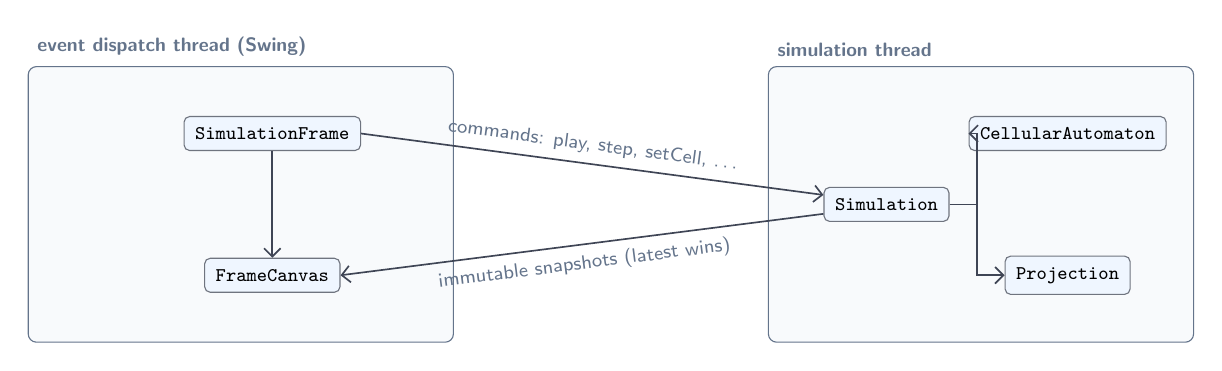
\begin{tikzpicture}[
      lane/.style={draw=muted, fill=packfill, rounded corners=3pt, minimum width=5.4cm,
        minimum height=3.5cm},
      item/.style={draw=ink!60, fill=classfill, rounded corners=2pt, font=\ttfamily\scriptsize,
        inner sep=4pt, align=center},
      flow/.style={-{Straight Barb[length=3pt]}, line width=0.6pt, draw=ink!80},
      note/.style={font=\sffamily\scriptsize, text=muted, align=center}]
    \node[lane] (edt) at (0, 0) {};
    \node[lane] (sim) at (9.4, 0) {};
    \node[packagelabel, anchor=south west] at (edt.north west) {event dispatch thread (Swing)};
    \node[packagelabel, anchor=south west] at (sim.north west) {simulation thread};
    \node[item] (frame) at (0.4, 0.9) {SimulationFrame};
    \node[item] (canvas) at (0.4, -0.9) {FrameCanvas};
    \node[item] (simulation) at (8.2, 0) {Simulation};
    \node[item] (automaton) at (10.5, 0.9) {CellularAutomaton};
    \node[item] (projection) at (10.5, -0.9) {Projection};
    \draw[flow] (frame) -- (canvas);
    \draw[flow] (simulation.east) -- ++(0.35, 0) |- (automaton.west);
    \draw[flow] (simulation.east) -- ++(0.35, 0) |- (projection.west);
    \draw[flow] (frame.east) -- node[note, above, sloped] {commands: play, step, setCell, \dots}
      ($(simulation.west)+(0,0.12)$);
    \draw[flow] ($(simulation.west)+(0,-0.12)$) -- node[note, below, sloped]
      {immutable snapshots (latest wins)} (canvas.east);
  \end{tikzpicture}
  \caption{Threading model. The automaton and its grid are only ever touched by the simulation
    thread; the two threads exchange commands in one direction and immutable snapshots in the
    other.}
  \label{fig:threads}
\end{figure}

The window is an Observer of the simulation. Its listener is called on the simulation thread and
does one thing: hand the snapshot to the event dispatch thread. If snapshots arrive faster than
Swing can paint, the intermediate ones are dropped and only the latest is shown, so a simulation
running flat out never floods the interface:

\begin{lstlisting}
private void enqueue(Snapshot snapshot) {              // called on the simulation thread
    if (pending.getAndSet(snapshot) == null) {
        SwingUtilities.invokeLater(this::showPending);
    }
}
\end{lstlisting}

\begin{figure}[tbp]
  \centering
  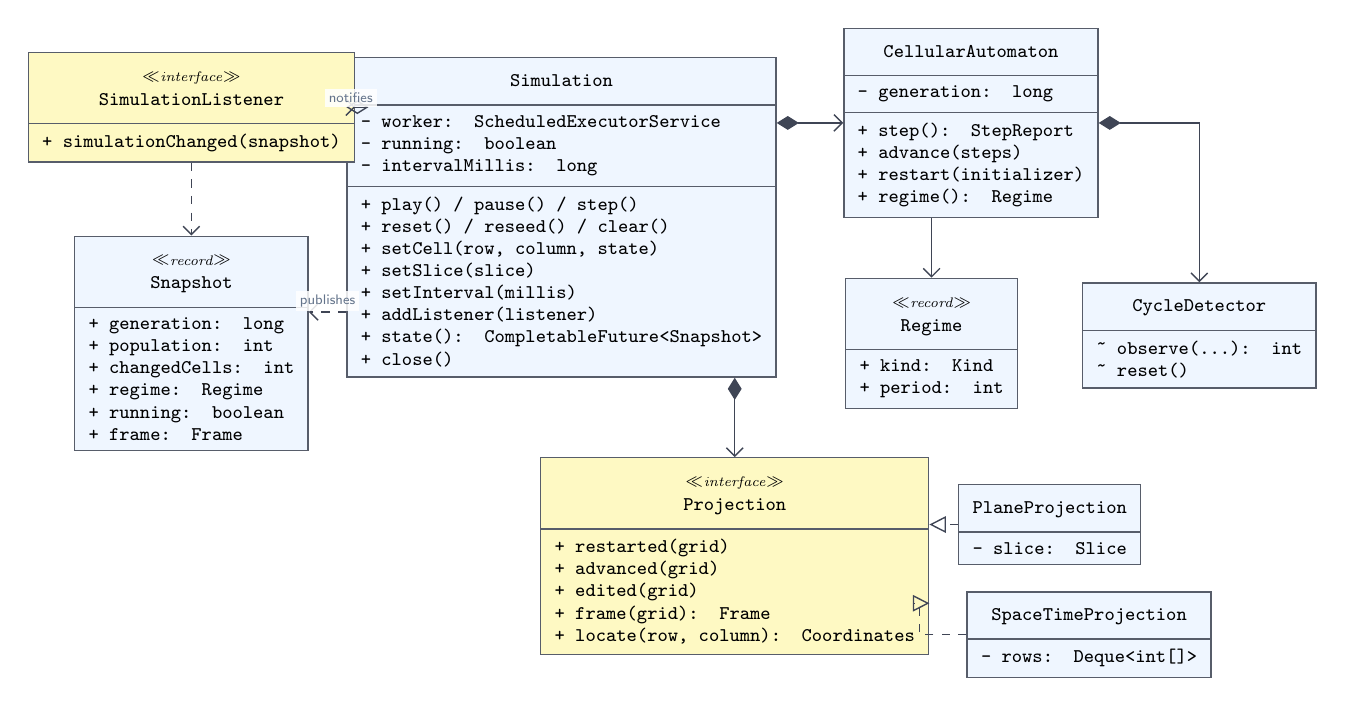
\begin{tikzpicture}
    \node[class=3] (sim) at (0, 0) {\ctitle{Simulation}
      \nodepart{second}- worker: ScheduledExecutorService\\- running: boolean\\
        - intervalMillis: long
      \nodepart{third}+ play() / pause() / step()\\+ reset() / reseed() / clear()\\
        + setCell(row, column, state)\\+ setSlice(slice)\\+ setInterval(millis)\\
        + addListener(listener)\\+ state(): CompletableFuture<Snapshot>\\+ close()};
    \node[iface] (listener) at (-4.7, 1.4) {\ctitle[interface]{SimulationListener}
      \nodepart{second}+ simulationChanged(snapshot)};
    \node[class] (snapshot) at (-4.7, -1.6) {\ctitle[record]{Snapshot}
      \nodepart{second}+ generation: long\\+ population: int\\+ changedCells: int\\
        + regime: Regime\\+ running: boolean\\+ frame: Frame};
    \node[class=3] (automaton) at (5.2, 1.2) {\ctitle{CellularAutomaton}
      \nodepart{second}- generation: long
      \nodepart{third}+ step(): StepReport\\+ advance(steps)\\+ restart(initializer)\\
        + regime(): Regime};
    \node[class] (cycles) at (8.1, -1.5) {\ctitle{CycleDetector}
      \nodepart{second}\textasciitilde{} observe(...): int\\\textasciitilde{} reset()};
    \node[class] (regime) at (4.7, -1.6) {\ctitle[record]{Regime}
      \nodepart{second}+ kind: Kind\\+ period: int};
    \node[iface] (projection) at (2.2, -4.3) {\ctitle[interface]{Projection}
      \nodepart{second}+ restarted(grid)\\+ advanced(grid)\\+ edited(grid)\\+ frame(grid): Frame\\
        + locate(row, column): Coordinates};
    \node[class] (plane) at (6.2, -3.9) {\ctitle{PlaneProjection}\nodepart{second}- slice: Slice};
    \node[class] (spacetime) at (6.7, -5.3) {\ctitle{SpaceTimeProjection}
      \nodepart{second}- rows: Deque<int[]>};

    \draw[aggregation] ($(sim.west)+(0,1.4)$) -- node[elabel, above] {notifies} (listener.east);
    \draw[uses] ($(sim.west)+(0,-1.2)$) -- node[elabel, above] {publishes}
      (snapshot.east |- {$(sim.west)+(0,-1.2)$});
    \draw[uses] (listener) -- (snapshot);
    \draw[composition] ($(sim.east)+(0,1.2)$) -- (automaton.west |- {$(sim.east)+(0,1.2)$});
    \draw[composition] (automaton.east) -| (cycles.north);
    \draw[association] (automaton.south -| regime.north) -- (regime.north);
    \draw[composition] (sim.south -| projection.north) -- (projection.north);
    \draw[implements] (plane.west) -- (plane.west -| projection.east);
    \draw[implements] (spacetime.west) -- ++(-0.6, 0) |- ($(projection.east)+(0,-0.6)$);
  \end{tikzpicture}
  \caption{The \code{automaton} and \code{simulation} packages.}
  \label{fig:simulation}
\end{figure}

\subsection{From a grid to a picture}

The subject asks for two displays. \code{Projection} is the interface behind both, a Strategy
chosen from the dimension of the grid:

\begin{itemize}
  \item \code{SpaceTimeProjection}, for one dimension, keeps the last 1\,024 generations and
    stacks them: this is the ``juxtaposition of successive states'' in which rule 18 draws the
    Sierpi\'nski triangle;
  \item \code{PlaneProjection}, for two dimensions and more, shows the current generation
    through a \code{Slice}, which can be moved while the simulation runs.
\end{itemize}

Both produce a \code{Frame}. The window, the PNG export and the text output all draw frames, so
the three share one rendering path and the exported picture is exactly what was on screen.

\subsection{The windows}

The interface is written with Swing and consists of two windows.

The \textbf{menu} (\cref{fig:launcher}) is the start-up screen required by the subject. It lists
the definition files of the current directory, or of another one, with what each describes.
Invalid files are listed in red with the reason of their rejection.

\begin{figure}[H]
  \centering
  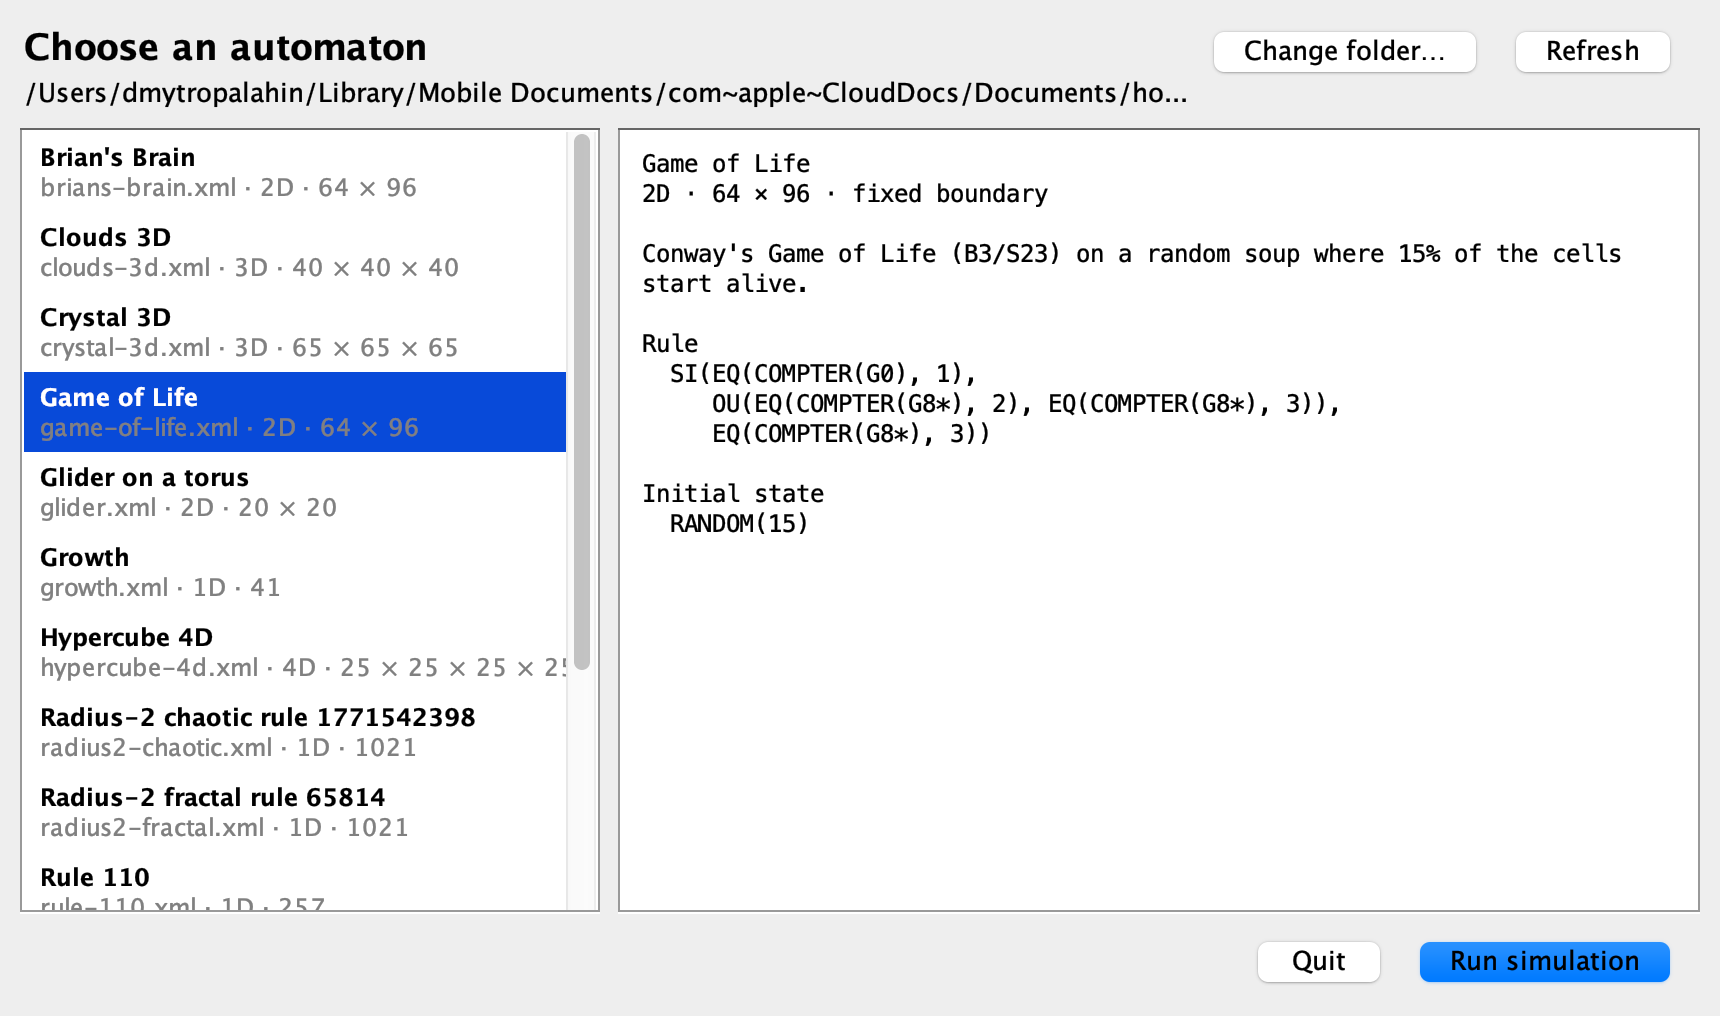
\includegraphics[width=0.74\textwidth]{launcher}
  \caption{The menu of the definition files of a directory.}
  \label{fig:launcher}
\end{figure}

The \textbf{simulation window} (\cref{fig:window}) shows one automaton. A toolbar gives the
commands (play or pause, single step, reset, new random draw, clear, speed, PNG export), a status
bar gives the generation, the population, the number of cells changed by the last step and the
regime. Clicking or dragging on the picture switches cells on and off, which makes it easy to
try a glider by hand. For a grid of three dimensions or more, a bar shows the slice in the
notation of the subject, with one spinner per pinned axis to move the plane.

\begin{figure}[H]
  \centering
  \begin{subfigure}[b]{0.43\textwidth}
    \centering
    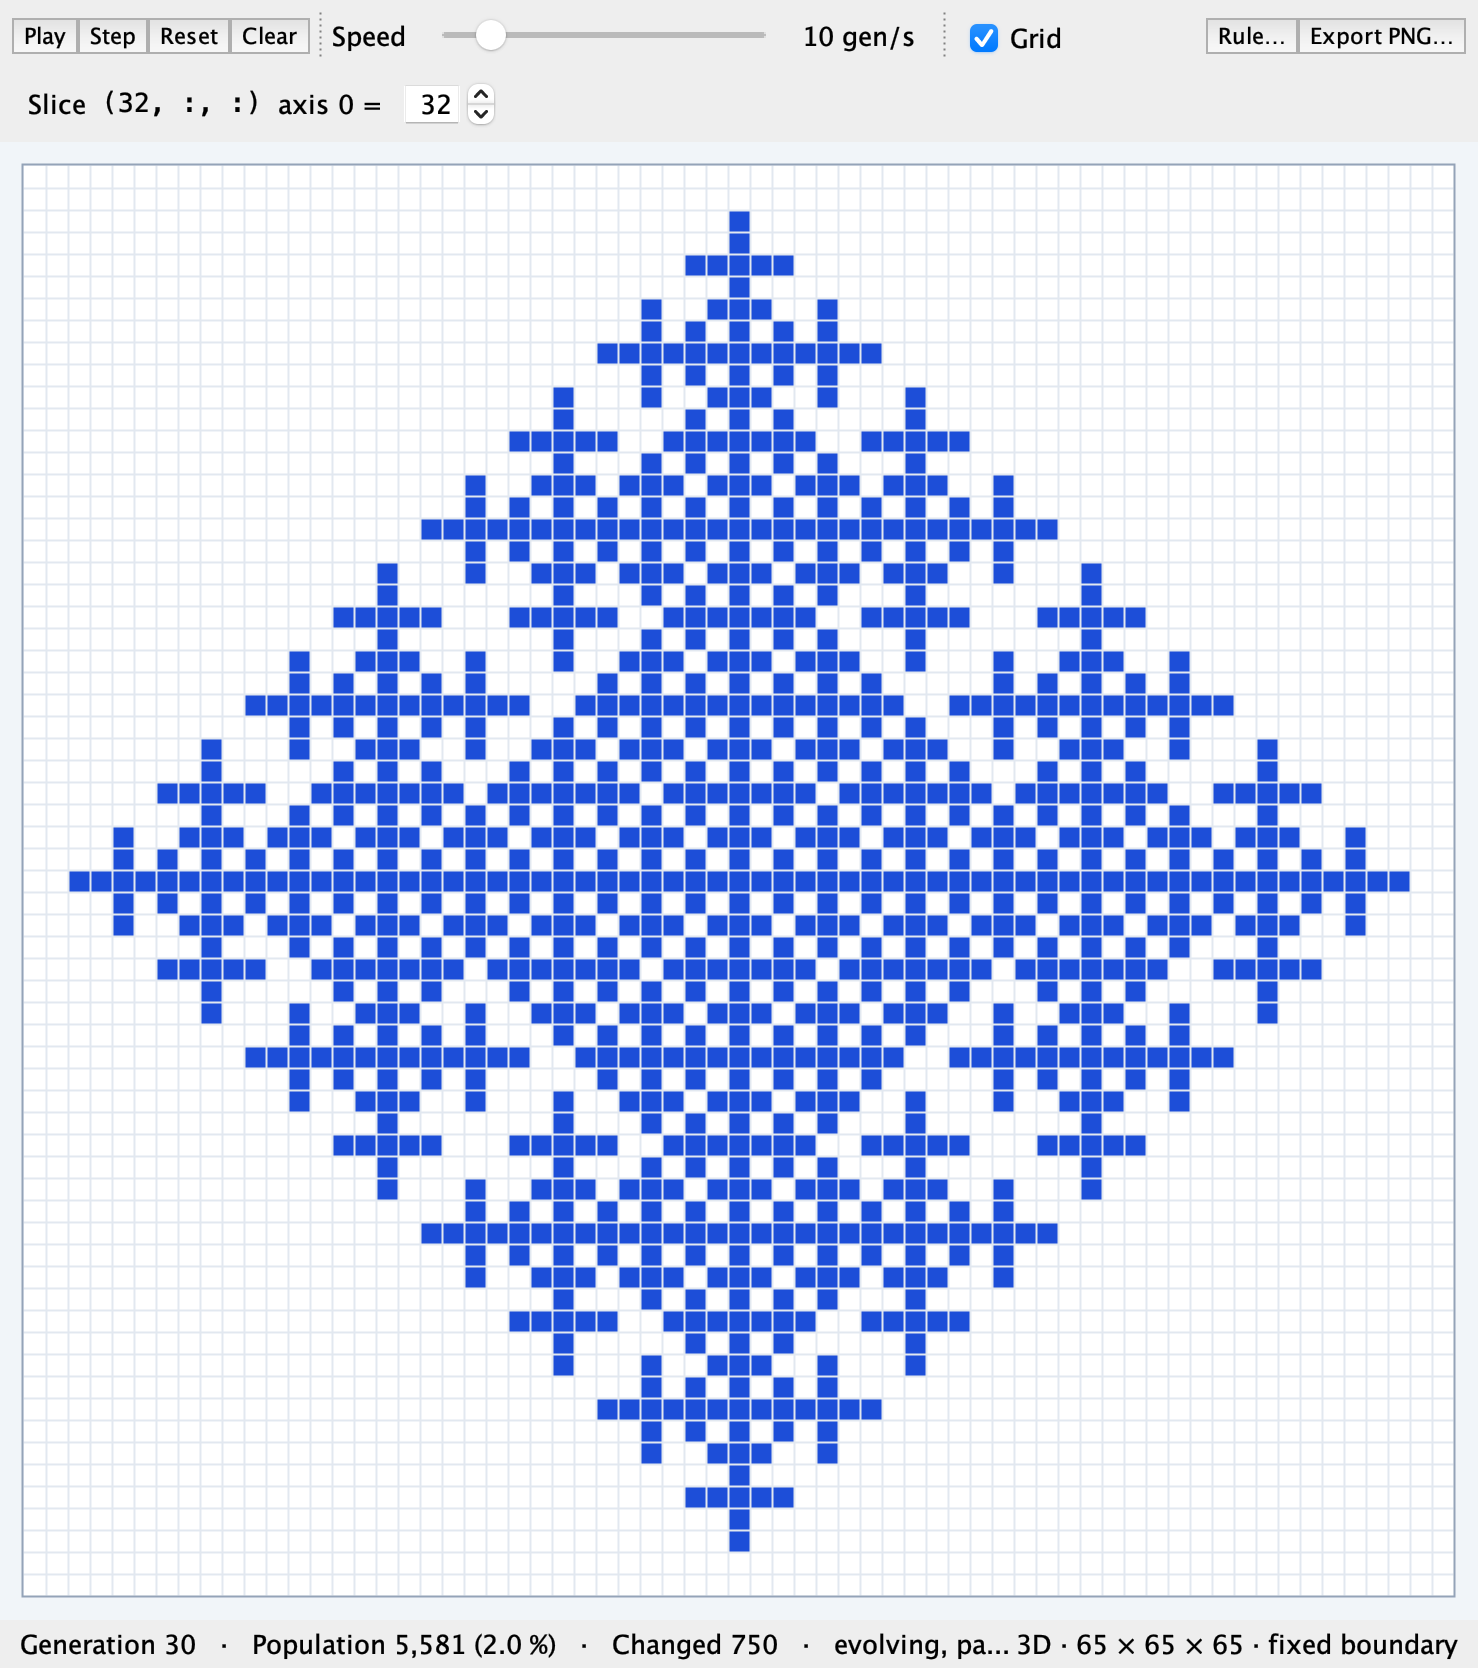
\includegraphics[width=\textwidth]{window-crystal-3d}
    \caption{A 3D automaton seen through the plane \code{(32, :, :)}}
  \end{subfigure}\hfill
  \begin{subfigure}[b]{0.55\textwidth}
    \centering
    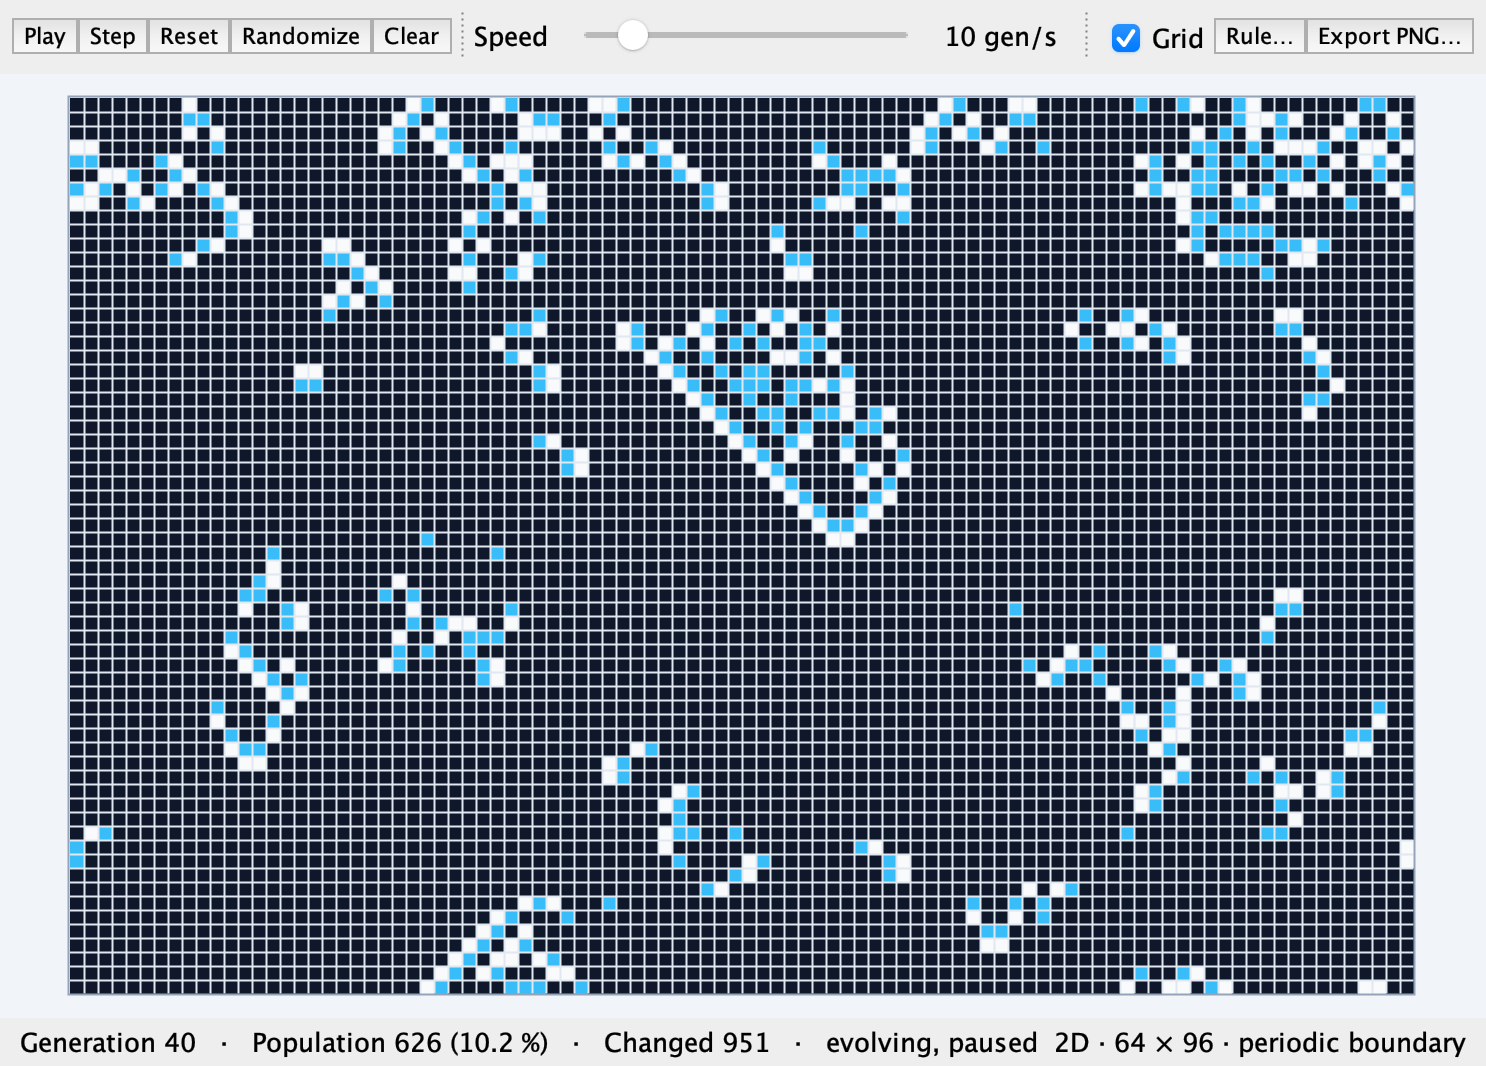
\includegraphics[width=\textwidth]{window-brians-brain}
    \caption{Brian's Brain, a three-state automaton with custom colors}
  \end{subfigure}
  \caption{The simulation window.}
  \label{fig:window}
\end{figure}

The drawing itself is done by \code{FrameCanvas}. A frame is first rendered at one pixel per
cell into an image, with a table lookup per cell, then magnified by the graphics library with
nearest-neighbor interpolation. Repainting a million cells is thus one array pass and one image
blit.

\subsection{Without a display}

Everything the windows do is also available from the command line (\cref{tab:commands}), through
the same classes. The command-line interface is what made it possible to test the application end
to end on a build server, and to produce the figures of this report with the program itself.
When no display is available, the menu falls back to a numbered list in the terminal.

\begin{table}[H]
  \centering\small
  \begin{tabularx}{0.92\textwidth}{@{}l L@{}}
    \toprule
    Command & Effect \\
    \midrule
    \code{menu} (default) & List the definition files of a directory and launch one \\
    \code{run FILE} & Open the simulation window of one file \\
    \code{list}, \code{validate FILE...} & Print the files of a directory; check files and
      explain what is wrong \\
    \code{print FILE}, \code{render FILE} & Run an automaton and output the result as text, or as
      a PNG image \\
    \code{explore} & Search for fractal or chaotic rules of radius 2 (\cref{sec:bonus}) \\
    \bottomrule
  \end{tabularx}
  \caption{The commands of the application.}
  \label{tab:commands}
\end{table}

\section{Bonus question: a rule of radius 2}
\label{sec:bonus}

\subsection{The question}

The bonus question asks to \emph{use the implementation} to find a one-dimensional automaton
whose juxtaposed states draw a fractal or chaotic figure, with a rule that considers the two
cells to the left of the current cell and the two cells to its right. The figure must not be
obtainable with the left, current and right cells alone. There are $2^{2^5} = 2^{32}$ such rules,
about four billion.

\subsection{Method}

\paragraph{A fast simulator for a narrow problem.} The general engine evaluates a syntax tree
for every cell: it runs \emph{one} automaton of any dimension well, but trying thousands of rules
calls for something leaner. A two-state rule of radius 2 is entirely described by its truth
table, 32 output bits, hence a 32-bit number. \code{TableRule} stores that number and computes a
generation with one table lookup per cell, sliding a five-bit window along the row.

\paragraph{Families instead of four billion rules.} \code{RuleExplorer} explores three families:
the 64 \emph{totalistic} rules, whose result only depends on how many of the five cells are on,
exhaustively; and random samples of the $2^{20}$ left-right \emph{symmetric} rules or of all
rules. Rules that switch cells on in an empty row are skipped, since their whole background
flickers.

\paragraph{Measuring a picture.} Each rule is run for 255 generations from a single live cell,
on a row wide enough for the pattern never to reach the edges. The resulting picture is measured
in two ways.

\begin{itemize}
    \item The \emph{box-counting dimension}. Cover the picture with boxes of side $s$ and count
          those containing a live cell, $N(s)$. For a fractal, $N(s) \propto s^{-D}$; $D$ is estimated
          as the slope of the least-squares line through the points $(\log 1/s, \log N(s))$ for
          $s = 2, 4, \dots, 32$. A line has dimension 1, a filled area 2, and the Sierpi\'nski triangle
          $\log 3 / \log 2 \approx 1.585$.
    \item The \emph{compression ratio}. The cells are packed eight to a byte and deflated; the
          ratio of the compressed size to the packed size is close to 0 for uniform or periodic
          pictures, small for nested ones, and large for disordered ones.
\end{itemize}

The two numbers place a picture in one of four classes: \emph{extinct} (the last row is empty),
\emph{regular}, \emph{fractal} (dimension between 1.25 and 1.85) or \emph{chaotic} (dimension
above 1.85 and compression ratio above 0.30). The thresholds were calibrated on radius-1 rules
whose behavior is well known (\cref{tab:calibration}). The program measures $D = 1.585$ for rule
18, the theoretical value to three decimals, which validates the estimator.

\begin{table}[H]
    \centering\small
    \begin{tabular}{@{}lccl@{}}
        \toprule
        Radius-1 rule            & Dimension & Compression & Verdict \\
        \midrule
        4 (a lone cell persists) & 1.000     & 0.005       & regular \\
        254 (filled triangle)    & 1.962     & 0.057       & regular \\
        18 and 90 (Sierpi\'nski) & 1.585     & 0.061       & fractal \\
        150                      & 1.695     & 0.081       & fractal \\
        30                       & 1.944     & 0.386       & chaotic \\
        45                       & 1.988     & 0.587       & chaotic \\
        \bottomrule
    \end{tabular}
    \caption{Calibration of the classifier on elementary rules.}
    \label{tab:calibration}
\end{table}

This classification is a filter, not a proof: it shortlists candidates, and the final choice is
made by looking at the pictures.

\paragraph{Making sure radius 2 is needed.} A candidate is kept only if (1) its truth table
depends on at least one of the two outer cells, and (2) its picture differs from the picture of
\emph{each of the 256 rules of radius 1} run from the same row. The second test is what the
question literally asks.

\paragraph{Back to the general engine.} A rule worth keeping is translated into the rule
language: a totalistic rule becomes tests on \code{COMPTER} over the five cells, any other rule a
decision tree of \code{SI} operators over one-cell neighborhoods. The result is written as a
definition file and is, from then on, an automaton like any other. A test runs the fast simulator
and the general engine side by side on random radius-2 rules and checks that they agree on every
cell of every generation, so the two implementations validate each other.

\subsection{Results}

The command \code{cellula explore --write examples} explores the totalistic family in about a
second and reports 7 fractal and 6 chaotic rules that genuinely need radius 2. The best of each
kind (\cref{tab:bonus}, \cref{fig:bonus}) ships with the project as
\code{examples/radius2-fractal.xml} and \code{examples/radius2-chaotic.xml}.

\begin{table}[H]
    \centering\small
    \begin{tabularx}{\textwidth}{@{}l L L@{}}
        \toprule
                               & Fractal                                            & Chaotic          \\
        \midrule
        Rule, in words         & on when \emph{exactly one} of the five cells is on &
        on when \emph{one, two or four} of the five cells are on                                       \\
        Rule language          & \code{EQ(COMPTER(G4), 1)}                          &
        \code{OU(EQ(COMPTER(G4), 1), OU(EQ(COMPTER(G4), 2), EQ(COMPTER(G4), 4)))}                      \\
        Wolfram code           & 65\,814                                            & 1\,771\,542\,398 \\
        Box-counting dimension & 1.50                                               & 1.95             \\
        Compression ratio      & 0.03                                               & 0.43             \\
        \bottomrule
    \end{tabularx}
    \caption{The two rules retained, with
        $G4 = \{(-2), (-1), (0), (1), (2)\}$ declared in the files.}
    \label{tab:bonus}
\end{table}

\begin{figure}[H]
    \centering
    \begin{subfigure}[b]{\textwidth}
        \centering
        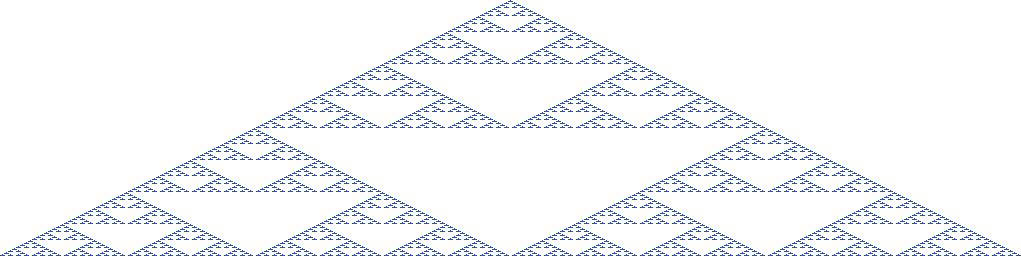
\includegraphics[width=0.92\textwidth]{radius2-fractal}
        \caption{Fractal: \code{EQ(COMPTER(G4), 1)}}
    \end{subfigure}\\[0.8em]
    \begin{subfigure}[b]{\textwidth}
        \centering
        
\includegraphics[width=0.92\textwidth]{radius2-chaotic}
        \caption{Chaotic: one, two or four live cells among the five}
    \end{subfigure}
    \caption{Generations 0 to 255 of the two radius-2 rules, from a single live cell, rendered by
        \code{cellula render}.}
    \label{fig:bonus}
\end{figure}

For these two rules there is also a one-line argument that no rule of radius 1 can draw the same
figure: their pattern widens by \emph{two} cells per generation on each side, whereas a rule of
radius 1 propagates information by at most one cell per generation.

Sampling 20\,000 rules of the symmetric or of the general family takes about eight seconds and
shortlists a few thousand candidates each; searches are reproducible thanks to a seed.

\section{Testing and measurements}
\label{sec:quality}

\subsection{Test strategy}

The project has 409 automated tests, written with JUnit and run by a single command,
\code{./mvnw verify}. They are of four kinds.

\begin{description}[leftmargin=1.2em,style=nextline]
  \item[Unit tests of the model.] Each class is tested through its public interface: the
    recursive array in one to six dimensions, the two boundary conditions, the truth table of
    every operator against its definition in the subject, the size and content of every
    predefined neighborhood in dimensions one to five.
  \item[Tests against the subject.] The figures of the subject are used as oracles. The growth
    automaton must reproduce figure 2 row by row; the Sierpi\'nski rule must match the truth table
    of figure 4 \emph{and} the arithmetic formula of the subject on every cell of 31 generations;
    the worked example of section 2.3 must parse to the expected tree. For the Game of Life, the
    classical patterns are checked: a block is stable, a blinker has period 2, a glider moves by
    one cell diagonally every four generations.
  \item[Cross-validation.] Two independent implementations of one-dimensional automata exist: the
    general engine and the fast simulator of the rule explorer. A test generates random rules,
    translates them from one representation to the other, and requires both to agree on every
    cell. A bug in either, or in the translation, would break it.
  \item[End-to-end tests.] The command-line interface is driven with real arguments in a
    temporary directory, and its output, exit status and generated files are checked: this
    exercises the whole chain from an XML file to a PNG image. The Swing windows have their own
    tests, which build the real windows without showing them and press their buttons; they need
    a display and are skipped on a build server.
\end{description}

Invalid inputs receive as much attention as valid ones: 27 kinds of invalid definition files and
18 kinds of syntax errors are each checked for the message shown to the user. Every file of the
\code{examples} directory is loaded and run by a test, so a broken example cannot be shipped.

\begin{table}[H]
  \centering\small
  \begin{tabular}{@{}lrrrrr@{}}
    \toprule
    Package & Classes & Lines & Tests & Line coverage & Branch coverage \\
    \midrule
    \code{grid} & 16 & 345 & 56 & 97\,\% & 94\,\% \\
    \code{neighborhood} & 5 & 148 & 63 & 99\,\% & 94\,\% \\
    \code{rule} (with \code{expression}, \code{parser}) & 28 & 279 & 93 & 100\,\% & 96\,\% \\
    \code{automaton} & 6 & 59 & 19 & 95\,\% & 95\,\% \\
    \code{config} & 16 & 358 & 95 & 97\,\% & 91\,\% \\
    \code{simulation} & 5 & 200 & 18 & 96\,\% & 83\,\% \\
    \code{render}, \code{ui.text} & 5 & 143 & 9 & 99\,\% & 85\,\% \\
    \code{explore} & 6 & 262 & 26 & 98\,\% & 92\,\% \\
    \code{cli} & 11 & 286 & 25 & 94\,\% & 89\,\% \\
    \midrule
    All of the above & 98 & 2\,080 & 404 & 97\,\% & 92\,\% \\
    \code{ui.swing} & 12 & 460 & 5 & \multicolumn{2}{c}{needs a display} \\
    \bottomrule
  \end{tabular}
  \caption{Tests and coverage by package, as measured by JaCoCo in a headless build. Classes
    include nested classes; lines are executable lines.}
  \label{tab:coverage}
\end{table}

\subsection{Tooling}

\begin{itemize}
  \item \textbf{Build.} Maven, through the wrapper, so that the only prerequisite is a JDK. The
    application itself has no dependency: only the tests need JUnit.
  \item \textbf{Compiler as reviewer.} The code is compiled with all the lints of \code{javac}
    enabled and treated as errors: an unchecked conversion or a missing case does not compile.
  \item \textbf{Continuous integration.} A GitHub Actions workflow builds and tests on Linux,
    macOS and Windows, with two versions of the JDK, and validates the example files with the
    packaged application.
  \item \textbf{Version control.} The history follows the Conventional Commits convention, one
    commit per coherent step of the work.
\end{itemize}

\subsection{Performance}

\Cref{tab:performance} gives the time needed to compute one generation. The cost is proportional
to the number of cells times the number of cells the rule reads; large grids use all the cores.
A million-cell Game of Life runs at about 35 generations per second, far beyond what the display
needs, which confirms that keeping the recursive array and an interpreted rule was affordable.

\begin{table}[H]
  \centering\small
  \begin{tabular}{@{}llrr@{}}
    \toprule
    Automaton & Neighborhood & Cells & Time per generation \\
    \midrule
    Sierpi\'nski, 1D & G2 & 257 & 0.02 ms \\
    Game of Life, $64 \times 96$ & G8* & 6\,144 & 0.8 ms \\
    Game of Life, $512 \times 512$ & G8* & 262\,144 & 7 ms \\
    Game of Life, $1024 \times 1024$ & G8* & 1\,048\,576 & 29 ms \\
    Crystal, $65^3$ & G6* & 274\,625 & 8 ms \\
    Clouds, $40^3$ & G26* & 64\,000 & 13 ms \\
    Hypercube, $25^4$ & G8* (4D) & 390\,625 & 18 ms \\
    \bottomrule
  \end{tabular}
  \caption{Median time per generation on an Apple M1~Pro (10 cores), OpenJDK 27. Grids below
    8\,192 cells are computed on a single thread.}
  \label{tab:performance}
\end{table}

\section{Conclusion}
\label{sec:conclusion}

\subsection{Summary}

Cellula meets every requirement of the subject: a recursive array whose dimension is chosen at
run time, neighborhoods exposed as traversals and definable by the user, the eleven operators
organized in a class hierarchy, an input file format, a graphical display for one, two and more
dimensions, a menu of the available files, the two required definitions, and an answer to the
bonus question obtained with the program itself.

Three design decisions proved the most valuable.

\begin{itemize}
    \item \emph{Letting the grid answer for every position.} Because \code{Grid.cellAt} always
          returns a cell, neither the neighborhoods nor the operators contain a single bounds check,
          and a second boundary condition was added by writing one method.
    \item \emph{Generating the neighborhoods instead of listing them.} Two formulas replace six
          special cases and make the program work in four dimensions without a line of
          dimension-specific code.
    \item \emph{Separating the definition from the automaton, and the automaton from its display.}
          The same classes serve the window, the terminal, the batch commands and the tests; this is
          what made it possible to test nearly everything automatically and to produce the figures of
          this report with the program.
\end{itemize}

\subsection{Limits}

\begin{itemize}
    \item \textbf{Repeated work in rules.} A rule such as the Game of Life mentions
          \code{COMPTER(G8*)} three times, and each occurrence walks the neighborhood again. Sharing
          identical sub-expressions when the tree is built would roughly halve the cost of such rules.
    \item \textbf{Memory.} Every cell is an object holding its coordinates. This is what the
          recursive, object-oriented design of the subject leads to, and it limits practical grids to
          a few million cells; a flat array of integers would use ten times less memory.
    \item \textbf{Display of higher dimensions.} A grid of three dimensions or more is only seen
          one plane at a time. A true 3D view would be a natural addition.
    \item \textbf{Cycle detection} is bounded to periods of at most 1\,024 generations, and relies
          on 64-bit fingerprints: a collision is extremely unlikely but not impossible.
    \item \textbf{The classification of pictures} in the rule explorer is a heuristic. It
          shortlists candidates well, but a human still chooses among them.
\end{itemize}

\subsection{Possible extensions}

The architecture leaves clear places for further work: new operators are one class and one line
of registration (\code{MOD}, or a count of cells in an arbitrary state, would make multi-state
automata such as Wireworld concise); a new boundary condition is one constant; another input
format only has to produce an \code{AutomatonDefinition}; and a new display is another
implementation of \code{Projection} or another listener of the simulation.


\appendix
\section{Building and running}
\label{app:usage}

The only prerequisite is a JDK, version 21 or newer.

\begin{lstlisting}[style=text]
./mvnw package                                    build target/cellula.jar and run the tests
java -jar target/cellula.jar --dir examples       open the menu on the example files
java -jar target/cellula.jar help                 list the commands
\end{lstlisting}

Without arguments, the program lists the definition files of the current directory, as the
subject requires. In the simulation window, the space bar plays or pauses, the right arrow
advances by one generation, and \code{R} goes back to generation 0.

\begin{lstlisting}[style=text]
java -jar target/cellula.jar print examples/sierpinski.xml --steps 31
java -jar target/cellula.jar render examples/crystal-3d.xml --steps 30 --output crystal.png
java -jar target/cellula.jar validate examples/*.xml
java -jar target/cellula.jar explore --family symmetric --samples 50000 --write found
\end{lstlisting}

\section{Reference of the rule language}
\label{app:language}

\begin{lstlisting}[style=text]
rule         := expression
expression   := NUMBER | NAME '(' arguments ')'
arguments    := neighborhood | [ expression { ',' expression } ]
neighborhood := NAME
NUMBER       := '-'? DIGIT+
NAME         := LETTER ( LETTER | DIGIT | '_' )* '*'?
\end{lstlisting}

\begin{table}[H]
    \centering\small
    \begin{tabularx}{\textwidth}{@{}l L l@{}}
        \toprule
        Operator                                             & Value                                                               & Alias        \\
        \midrule
        \code{ET(a, b)}                                      & 1 if \code{a} and \code{b} are both different from 0, else 0        & \code{AND}   \\
        \code{OU(a, b)}                                      & 0 if \code{a} and \code{b} are both equal to 0, else 1              & \code{OR}    \\
        \code{NON(a)}                                        & 1 if \code{a} equals 0, else 0                                      & \code{NOT}   \\
        \code{SUP(a, b)}                                     & 1 if \code{a} is strictly greater than \code{b}, else 0             & \code{GT}    \\
        \code{SUPEQ(a, b)}                                   & 1 if \code{a} is greater than or equal to \code{b}, else 0          & \code{GE}    \\
        \code{EQ(a, b)}                                      & 1 if \code{a} equals \code{b}, else 0                               &              \\
        \code{COMPTER(G)}                                    & number of cells in state 1 in the neighborhood \code{G} of the cell &
        \code{COUNT}                                                                                                                              \\
        \code{ADD(a, b)}, \code{SUB(a, b)}, \code{MUL(a, b)} & sum, difference, product                                            &              \\
        \code{SI(c, a, b)}                                   & \code{a} if \code{c} is different from 0, else \code{b}             & \code{IF}    \\
        \code{ETAT()}                                        & state of the cell itself (extension)                                & \code{STATE} \\
        \bottomrule
    \end{tabularx}
    \caption{The operators of the rule language.}
\end{table}

\section{The example files}
\label{app:examples}

\begin{table}[H]
    \centering\small
    \begin{tabularx}{\textwidth}{@{}l l L@{}}
        \toprule
        File                                                   & Grid           & Demonstrates                                            \\
        \midrule
        \code{game-of-life.xml}                                & $64 \times 96$ & Required: Game of Life from \code{RANDOM(15)}           \\
        \code{sierpinski.xml}                                  & 257            & Required: Sierpi\'nski triangle, formula of the subject \\
        \code{growth.xml}                                      & 41             & Figures 1 and 2 of the subject                          \\
        \code{subject-example.xml}                             & $64 \times 96$ & The rule of section 2.3, verbatim                       \\
        \code{glider.xml}                                      & $20 \times 20$ & Explicit cells, periodic boundary, cycle detection      \\
        \code{rule-30.xml}, \code{rule-110.xml}                & 257            & User-defined one-cell neighborhoods                     \\
        \code{brians-brain.xml}                                & $64 \times 96$ & Three states, colors, \code{ETAT()}                     \\
        \code{snowflake.xml}                                   & $97 \times 97$ & Hexagonal lattice by a user-defined neighborhood        \\
        \code{crystal-3d.xml}                                  & $65^3$         & Three dimensions, G6*, slice \code{(32, :, :)}          \\
        \code{clouds-3d.xml}                                   & $40^3$         & Three dimensions, G26*, random start                    \\
        \code{hypercube-4d.xml}                                & $25^4$         & Four dimensions, slice \code{(:, :, 12, 12)}            \\
        \code{radius2-fractal.xml}, \code{radius2-chaotic.xml} & 1\,021         & Bonus question                                          \\
        \bottomrule
    \end{tabularx}
    \caption{The definition files shipped with the project.}
\end{table}

\begin{figure}[H]
    \centering
    \begin{subfigure}[b]{0.31\textwidth}
        \centering
\includegraphics[width=\textwidth]{snowflake}
        \caption{\code{snowflake.xml}}
    \end{subfigure}\hfill
    \begin{subfigure}[b]{0.31\textwidth}
        \centering
\includegraphics[width=\textwidth]{hypercube-4d}
        \caption{\code{hypercube-4d.xml}}
    \end{subfigure}\hfill
    \begin{subfigure}[b]{0.31\textwidth}
        \centering
\includegraphics[width=\textwidth]{clouds-3d}
        \caption{\code{clouds-3d.xml}}
    \end{subfigure}\\[0.8em]
    \begin{subfigure}[b]{0.48\textwidth}
        \centering
\includegraphics[width=\textwidth]{rule-30}
        \caption{\code{rule-30.xml}}
    \end{subfigure}\hfill
    \begin{subfigure}[b]{0.48\textwidth}
        \centering
\includegraphics[width=\textwidth]{subject-example}
        \caption{\code{subject-example.xml}}
    \end{subfigure}
    \caption{A few of the examples, rendered by \code{cellula render}.}
\end{figure}


\end{document}
